\documentclass[12pt,onecolumn]{article}
\usepackage{graphicx}
\usepackage{hyperref}
\usepackage{url}
\usepackage{wrapfig}
\usepackage{listings}
\usepackage{tikz}
\usepackage{caption}
\usepackage{subcaption}
\usetikzlibrary{shapes}
\usetikzlibrary{positioning}
\usepackage{pdfpages}
\usepackage{longtable}
\usepackage[title]{appendix}
\usepackage{array}
\usepackage{caption}
\usepackage{capt-of}
\newcommand{\horrule}[1]{\rule{\linewidth}{#1}}

\setlength{\parindent}{0em}
\setlength{\parskip}{0.5em}

\title{\huge Tracking Interconnected Facebook Links - Project Report}

\author{ \horrule{1pt} \\ \textbf{ELEN4009 - Software Engineering} \\ \emph{School of Electrical and Information Engineering,} \\ \emph{University of the Witwatersrand,} \\ \emph{Johannesburg, South Africa} \\ \horrule{1pt} \\\\ \emph{Back-End Pair:} \\ Julian Zeegers (704582) \\ James Allingham (672732) \\ \\ \emph{Front-End Pair:} \\ Joseph Gage (751052)\\ Nathan Haag (873666) \\ \horrule{1pt}}

\addtolength{\oddsidemargin}{-0cm}
\addtolength{\evensidemargin}{-.0cm}
\addtolength{\textwidth}{0cm}


%%%%%%%%%%%%%%%%%%%%%%%%%%%%%%%%%%%%%%%%%%%%%%%%%%%%%%%%%%%%%%%%%%%%%%%%%%%%%%%
\begin{document}
	
	\date{\vspace{-5ex}}
	\maketitle
	\pagestyle{plain}
	\thispagestyle{empty}
	
	\begin{abstract}
		The Tracking Facebook Interconnected Links project is fully documented after the first prototype is developed. A detailed Software Requirement Specification is described that covers both the back-end and front-end requirements. The front-end and back-end's design and implementation of the first increment of the project is discussed in detail as well as the goals that were achieved. The agile Scrum methodology approach that was used for this project is also reviewed with a full description of the first sprint of the project. The sprint retrospective summarizes the achievements of the first sprint and the improvements that can be made in the next sprint. 
	\end{abstract}
	
	\newpage
	
	\tableofcontents
	\listoffigures
	\listoftables
	\thispagestyle{empty}
	\setcounter{page}{0}
	
	\newpage
	
	\section{Introduction}
	
	\subsection{Problem Statement} % James
	
	Facebook is one of the most popular social networks used today. Due to the fact that it has over 1.5 billion users, it produces an incredibly large amount of data \cite{fb}. This data could be used in a number of ways, listed below.
	
	\begin{itemize}
		\item Data scientists and analysts could make use of this data to learn about social trends.
		
		\item Individuals can use the data for personal analytics.
		
		\item Sociologists to use the data to make and test new hypotheses.
		
		\item Marketing and advertising agencies could create specialized and targeted adds depending on a set of user's likes and status updates.
		
	\end{itemize}    
	
	There are a large number of potential applications and the possibilities are only constrained by human creativity.
	
	The Tracking Interconnected Facebook Links project is intended to visualize the links and connections of a Facebook user with other users. Initially, these visualisations are focused on identifying the relationships of a Facebook user (the end user of this product) with the network of friends this Facebook user has. The visuals are also intended to further illustrate the relationship connections of the user's friends of friends and an overview of the user's friend network. Some personal analytics such as analyses of the user's Facebook post contents will also be implemented. There is a myriad of additional features that could be added to this tool and therefore the solution must be dynamic and flexible. For example degrees of separation analyses or more personal analytics could be added. At a later point the project could be expanded to include the large scale data analytics used by data scientists, sociologists and marketers. 
	
	The project team consists of four Software Engineering students, divided into two groups: one for the front-end and one for the back-end. This document serves as a description of the project. The software requirement specification will be laid out. The design and implementation of the front and back ends will be discussed. Finally, the Scrum planning and retrospective will be presented.
	
	\subsection{Project Objectives} % James
	
	In order to both quantify the success of the project as well as properly create tasks with correct priorities, the objectives of the project must be laid out. They are as listed below.
	
	\begin{itemize}
		
		\item Create a prototype system for visualizing a person's Facebook connections, social trends and personal analytics.
		
		\item Document the requirements for the system.
		
		\item Document the design of the system.
		
		\item Document the implementation and testing of the system.
		
		\item Document the group work aspects of the system including the SDLC.
		
	\end{itemize}
	
	\subsection{Stakeholders} % James
	
	The Project Management Body of Knowledge describes stakeholders as individuals or organizations that may be impacted in any way by the decisions or outcomes of a project \cite{pmbok}. There are a number of stakeholders whose interests must be considered when carrying out the objectives above. Often the stakeholders can have conflicting interests which must be compared and carefully weighed up in order to resolve the conflict. The following stakeholders are considered to be of paramount importance:
	
	\begin{itemize}
		\item \textbf{The Users}. The users of the system will be individuals who wish to explore their own personal Facebook friend networks and perform intimate personal analytics on their data. At this point the users \textbf{do not} include data scientists, analysts, sociologists and marketing/ advertising professionals - a later version of the software will be targeted at these groups. The reason that the individual was chosen as the first target market is that the requirements for the individual are much less resource intensive and thus are a more realistic goal for the first version of a product. Every decision that is made should improve the user's experience when interacting with the product. 
		
		\item \textbf{The development team}. The development team consists of four software engineering students. These four developers are then divided into two teams, the front-end team and the back-end team. It is important that the work in the project is divided appropriately between the teams. Note that the Scrum SDLC does not make distinctions between different developers and so it is up to the developers themselves to choose the appropriate tasks that best fit their skill sets. The success or the failure of the project will have a large impact on the development team. On the other hand, the development team will have a large impact on whether or not the project is a success. Whenever a decision is made, it should be one that makes both the best use of the team as well as improves the likelihood that the project will be a success.
		
		\item \textbf{Facebook}. Although Facebook will not itself be involved in the project, the perception of the company could be influenced by the product if it is successful. This could be as a result of people learning more about amount or type of data about them on Facebook.
		
	\end{itemize}
	
	\subsection{Abbreviations, Acronyms and Definitions} % All of us
	
	\begin{enumerate}
		\item \textbf{ACID} - Atomicity Consistency Isolation Durability. A model for reliable database systems.
		
		\item \textbf{Apache}. A popular web server.
		
		\item \textbf{Client-Server}. An architecture or model for distributed computing via the Internet or other network.
		
		\item \textbf{CSS} - Cascading Style Sheets. A language for describing the presentation of a website.
		
		\item \textbf{Cypher}. The query language for Neo4j graph databases.
		
		\item \textbf{d3.js}. A popular JavaScript library for visualisation.
		
		\item \textbf{SVG}. Scalable Vector Graphic. An XML-based vector image format, supporting interactive functionality and animations.
		
		\item \textbf{DBMS} - Database Management System. A database program.
		
		\item \textbf{Django}. An MTV web application framework, written in Python.
		
		\item \textbf{Git}. A program for software and document version control.
		
		\item \textbf{GitHub}. A website for hosting git repositories.
		
		\item \textbf{GUI} - Graphical User Interface. A visual tool that allows a user to interact with an application.
		
		\item \textbf{HTML} - Hyper Text Markup Language. A language for creating web pages.
		
		\item \textbf{HTTP} - Hyper Text Transfer Protocol. An Application level protocol that makes use of HTML from sending and receiving messages in a client-server architecture.
		
		\item \textbf{JS} - JavaScript. A scripting language often used in building interactive applications in the Web 2.0.
		
		\item \textbf{JSON} - JavaScript Object Notation. A data interchange format used extensively in web applications.
		
		\item \textbf{mod\_wsgi}. The Django module for Apache Web Server.
		
		\item \textbf{MTV} - Model Template View. Another name for the popular MVC framework. This is the nomenclature used by the Django web framework.
		
		\item \textbf{MVC} - Model View Controller. A framework for building web applications based on a three layer abstraction of the data, the presentation and the interaction between them. 
		
		\item \textbf{Neo4j}. A graph database written in Java.
		
		\item \textbf{Py2Neo}. A Neo4j driver for the Python programming language.
		
		\item \textbf{Python}. A popular, powerful and flexible scripting language.
		
		\item \textbf{Slack}. An application for team communication.
		
		\item \textbf{SDLC} - Software Development Life Cycle. The process or approach the software development team adheres to.
		
		\item \textbf{SDD} - Software Design Description. A document detailing the design of a software project.
		
		\item \textbf{SVG} - Scalable Vector Graphic. A vector 2D image format.
		
		\item \textbf{Trello}. A web application for managing project tasks.
		
		\item \textbf{UI} - User Interface. A tool allowing a user to interact with an application.
		
		\item \textbf{Web 2.0}. The informal name for websites that emphasize user generated content such as Facebook.
		
		
	\end{enumerate}
	
	\section{Software Requirement Specification} % James
	
	\subsection{Introduction}
	This project is intended to visualise the links and connections of a Facebook user with other users. Initially, these visualisations are focused on identifying the relationships of a Facebook user (and the end user of this product) with the network of friends this Facebook user has. The visuals are also intended to further illustrate the relationship connections of the user's friends of friends and an overview of the user's friend network. Additional features could potentially be added to this tool and therefore the solution must be dynamic and flexible. This section describes the software requirements that will ensure that the end product is of the highest quality, produced most efficiently and fulfils its requirements.
	
	\subsubsection{Requirements}
	
	The requirements for the application are that it:
	\begin{enumerate}
		\item consists of a front-end that runs client side and a back-end that runs server side, 
		\item has user friendly front-end which is easy to use for non-technologically inclined people,
		\item is scalable - with a back-end that supports multiple clients,
		\item is fast and responsive leading to an enjoyable user experience,
		\item provides attractive and useful visualisations of Facebook data which allow the user to explore their Facebook networks in an intuitive and practical manner which facilitates discovery,
		\item is extensible - allowing for additions and modifications to be made quickly and with ease,
		\item is secure - keeping the users personal data safe and respecting their privacy, and
		\item allows flexibility for data acquisition - the application should allow users to upload their own data or access their data via the Facebook API.
	\end{enumerate}
	
	\subsubsection{Purpose}
	The purpose of the project is to provide a tool to be used by individuals (and organizations at a later stage) to learn more about friend networks and how people are connected. This could be for marketing purposes, sociological research, finding friends or even for personal  interest. Facebook provides a wealth of useful information about individuals, groups of individuals and companies. This project is a tool for visualizing this information dynamically so that it will be advantageous to any  user.
	
	\subsubsection{System Overview}
	This project will be made up of various software systems with the back-end and front-end working together to form a web-based visualisation application. The overview of the entire software system is illustrated in Figure \ref{system}. This figure shows how the various components of the system interact with each other. Figure \ref{system} shows how the client (using a web browser) interacts with an Apache server and the Django framework. It describes how data from the Neo4j database is fetched by the Django framework and sent to the user via the Apache server.
	
	\begin{figure}[h]
		\centering
		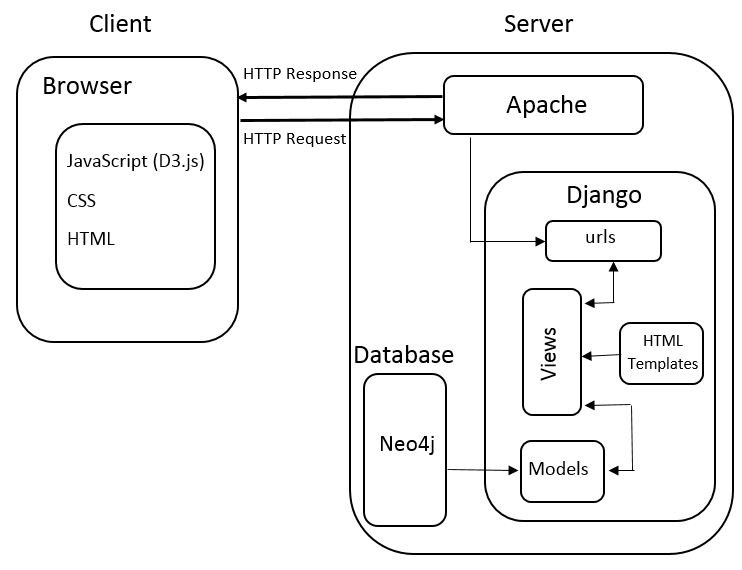
\includegraphics[width=\textwidth]{system}
		\caption{Diagram of System Overview}
		\label{system}
	\end{figure}
	
	\subsection{Software Development Life Cycle Choice}
	The SDLC is the process or approach the software development team adheres to throughout the project's development. Choosing the correct SDLC for the project is an important decision at the start of a software project as it could determine whether a project is successfully completed within the time frame, budget and scope requirements. A number of common SLDCs were considered and are listed below.
	
	\begin{itemize}
		\item \textbf{Waterfall model} - A sequential development model that lacks feedback. This technique consists of the following steps: requirements definition, design, implementation, verification and maintenance. However, due to the lack of feedback, this approach is not feasible unless the requirements are not completely defined in advance, the scope is fixed and the technology is well understood by the development team.
		
		\item \textbf{Iterative and Incremental process} - A development model in which features are gradually added. Unlike the waterfall approach, this approach makes small changes at a time which can allow for more flexibility. However, this approach still requires the whole system to be well defined at the project start.
		
		\item \textbf{Agile} - A number of development principles aimed at facilitating the evolution of requirements and solutions in a collaborative process.
		
	\end{itemize}
	
	For this particular project, the fast pace method of the Agile SDLC is the best approach as the pace of producing a working solution is a priority. The requirements for this project have not yet been fully defined and therefore the chosen Agile SDLC must be flexible and able to deal with requirement changes of various sizes.
	
	The Agile SDLC also has varying methodologies that allows the achievement of an agile software development movement. These methods include the Dynamic System Development Method, the Scrum Method, Rapid Application Development, extreme programming and the Feature-Driven Development Method. The Scrum methodology is the chosen method for this project as it allows the project progression to be agile and flexible with continuous feedback sessions to ensure the requirements are dynamically followed \cite{Kinsey}.
	
	In the Scrum process, prioritised project tasks (referred to as sprints) are defined in short daily meetings (typically 15 minutes) with all the project team members. These meetings allow the team to communicate project progress and identify the important features that need to be added in order to increase the project progress pace. For this project, these sprints will allow for a working product to be produced in the shortest amount of time while additional features can be  added at a later stage. This process also allows the client to closely keep track of progress and adjust the requirements in order to produce the most high-grade product possible. The daily meeting process occurs for up to 30 days by which time the first release of the developed software should be ready.   
	
	
	\subsection{Architecture Choice}
	The choice of software architecture is influenced by the tools and libraries used for both the front-end service and the back-end service (detailed in sections \ref{backsec} and \ref{frontsec}), network communication and team composition. 
	
	A two-tier, client-server architecture has been selected. In 'client-server', client refers to any user actively interacting with the server via the user interface provided by the system. Server refers to the storage and hosting of the business and data layers. The user interface is only possible with logic on the server. Based on user requests, the logic decides on the correct data to be sent from the server to the client. Having the logic stored on the same server as the database is an important step towards decreasing response time between receiving and fulfilling user request \cite{twotieradvantage}. 
	
	Two-tier means that any instance of a client utilizing the provided user interface will be separated from the server via a network through which all communication will occur. For the purpose of tracking interconnected Facebook links, the network between the client and the server will be the Internet. This design choice follows the need for multiple users to have access to the software simultaneously \cite{beginningsofteng}. 
	
	It is important to take note that in this architecture, the client and the server are tightly woven together, as communication between the two entities occurs directly over the network. This means that there is no middle tier to interpret and translate data correctly. In terms of team composition, this design choice is beneficial and reduces the amount of code needed to ensure compatibility.
	
	\subsection{Front-End Service} \label{frontsec}
	
	\subsubsection{User Interface Functionality}
	The front-end User Interface (UI) will contain several tools for visualizing Facebook friend networks. The most basic tool will show a simple network diagram to view all friends and friends of friends for the user. This friendship diagram will include several functionalities.
	
	Firstly, a user may select any of his friends and the diagram will transition to the selected person's friend network. This is pictured in Figure \ref{click}. 
	
	\begin{figure}[htbp]
		\centering	    
		\begin{subfigure}[b]{0.3\textwidth}
			\centering
			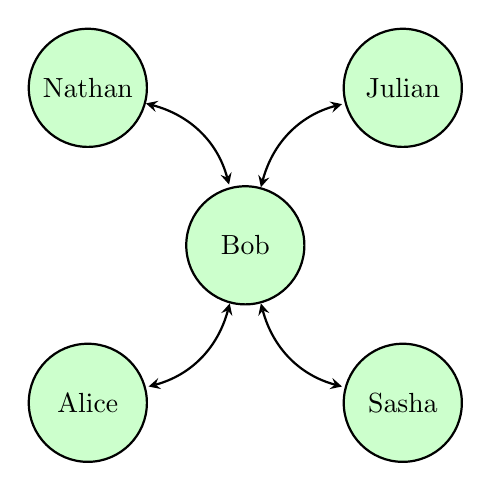
\begin{tikzpicture}[<->,>=stealth,shorten >=1pt,auto,thick,main node/.style={circle,fill=green!20,draw,align=center,minimum width=1.5cm}]
			
			\node[main node] at (2,0) (1) {Nathan};
			\node[main node] at (6,0) (2)  {Julian};
			\node[main node] at (4,-2) (3) {Bob};
			\node[main node] at (2,-4) (4) {Alice};
			\node[main node] at (6,-4) (5) {Sasha};	      
			
			\path
			(1) edge[bend left] (3)
			(3) edge[bend right] (5)
			(3) edge[bend left] (4)
			(3) edge[bend left] (2)   
			;
			
			\end{tikzpicture}
			\caption{Before click}
			\label{fig:gull1}
		\end{subfigure}
		\qquad
		\qquad
		\begin{subfigure}[b]{0.3\textwidth}
			\centering
			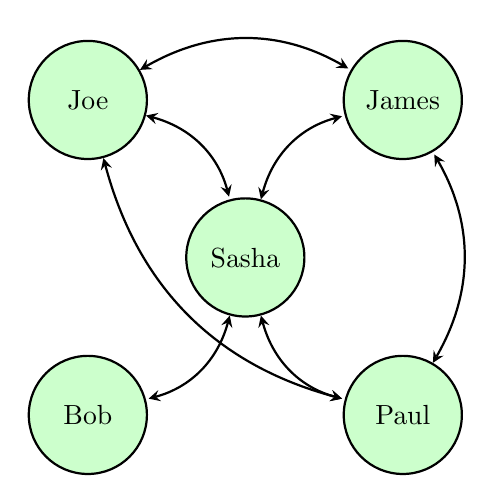
\begin{tikzpicture}[<->,>=stealth,shorten >=1pt,auto,thick,main node/.style={circle,fill=green!20,draw,align=center,minimum width=1.5cm}]
			
			\node[main node] at (10,0) (6) {Joe};
			\node[main node] at (14,0) (7) {James};
			\node[main node] at (12,-2) (8) {Sasha};
			\node[main node] at (14,-4) (9) {Paul};
			\node[main node] at (10,-4) (10) {Bob};      
			
			\path
			(6) edge[bend left] (8)
			(8) edge[bend right] (9)
			(8) edge[bend left] (10)
			(8) edge[bend left] (7)
			(9) edge[bend right] (7)
			(6) edge[bend right] (9)
			(6) edge[bend left] (7)
			;
			
			\end{tikzpicture}
			\caption{After click}
			\label{fig:gull2}
		\end{subfigure}
		\caption[Transition of friend network after clicking]{Transition of friend network after clicking on Sasha}
		\label{click}
	\end{figure}
	
	Secondly, the user may select certain information to be displayed on the diagram. For example, friendship data can be selected as in Figure \ref{details} or relationship data as in Figure \ref{relation}.
	
	\begin{figure}[htbp]
		\centering
		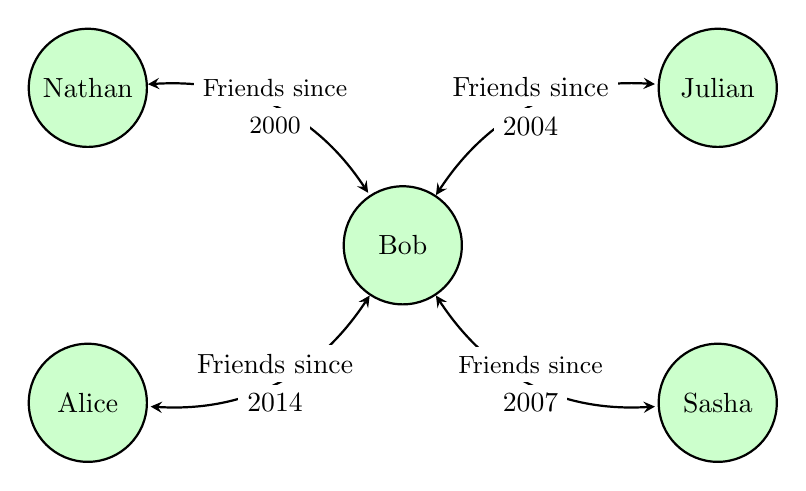
\begin{tikzpicture}[<->,>=stealth,shorten >=1pt,auto,thick,main node/.style={circle,fill=green!20,draw,align=center,minimum width=1.5cm}]
		
		\node[main node] at (0,0) (1) {Nathan};
		\node[main node] at (8,0) (2)  {Julian};
		\node[main node] at (4,-2) (3) {Bob};
		\node[main node] at (0,-4) (4) {Alice};
		\node[main node] at (8,-4) (5) {Sasha};
		
		\path
		(1) edge[bend left] node[above, fill=white] {\small Friends since} node[below,fill=white] {\small 2000} (3)
		(3) edge[bend right] node[above, fill=white] {\small Friends since} node[below,fill=white] {2007} (5)
		(3) edge[bend left] node[above,fill=white] {Friends since} node[below,fill=white] {2014} (4)
		(3) edge[bend left] node[above,fill=white] {Friends since} node[below,fill=white] {2004}(2)
		;
		
		\end{tikzpicture}
		\caption{Friend network showing friendship details.}
		\label{details}
	\end{figure}
	
	\begin{figure}[htbp]
		\centering
		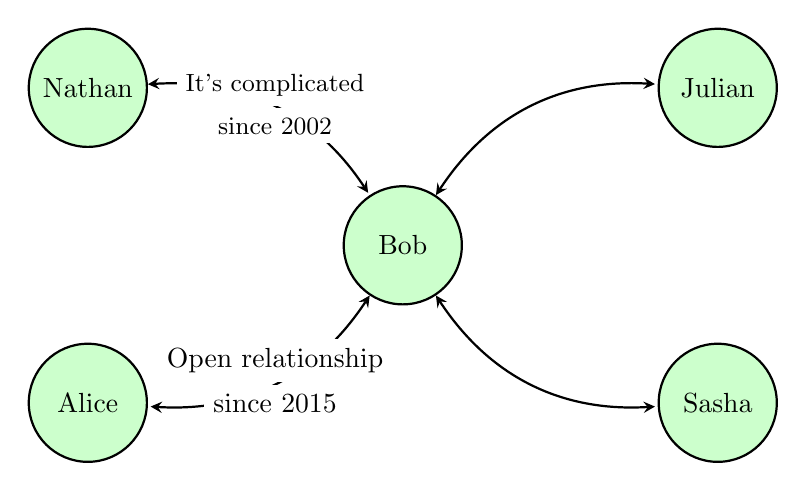
\begin{tikzpicture}[<->,>=stealth,shorten >=1pt,auto,thick,main node/.style={circle,fill=green!20,draw,align=center,minimum width=1.5cm}]
		
		\node[main node] at (0,0) (1) {Nathan};
		\node[main node] at (8,0) (2)  {Julian};
		\node[main node] at (4,-2) (3) {Bob};
		\node[main node] at (0,-4) (4) {Alice};
		\node[main node] at (8,-4) (5) {Sasha};
		
		\path
		(1) edge[bend left] node[above, fill=white] {\small It's complicated} node[below,fill=white] {\small since 2002} (3)
		(3) edge[bend right] (5)
		(3) edge[bend left] node[above,fill=white] {Open relationship} node[below,fill=white] {since 2015} (4)
		(3) edge[bend left] (2)
		;
		
		\end{tikzpicture}
		\caption{Friend network showing relationship details.}
		\label{relation}
	\end{figure}
	
	Thirdly, the user will be able to show additional information about a user such as their personal information. This is shown in Figure \ref{moreinfo}.
	
	\begin{figure}[htbp]
		\centering
		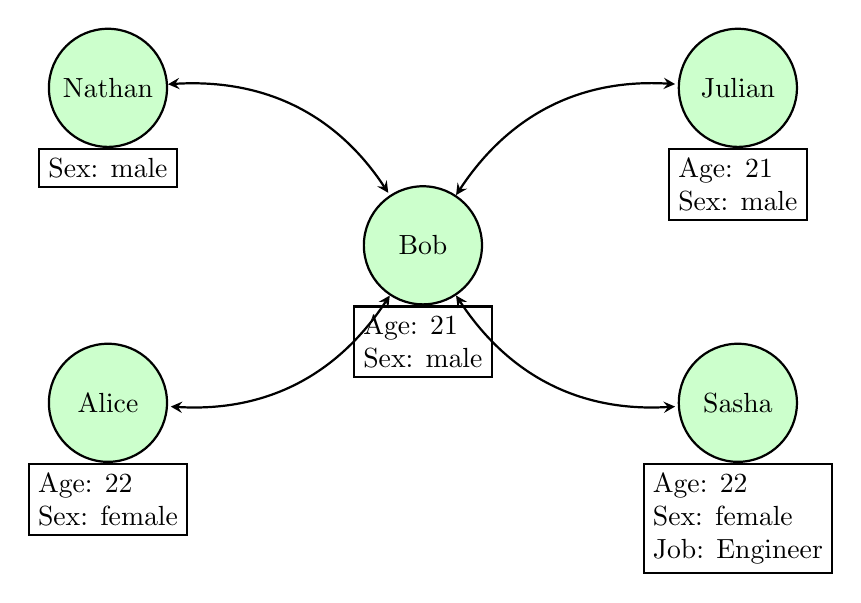
\begin{tikzpicture}[<->,>=stealth,shorten >=1pt,auto,thick,main node/.style={circle,fill=green!20,draw,align=center,minimum width=1.5cm}]
		
		\node[main node] at (0,0) (1) {Nathan};
		\node[main node] at (8,0) (2)  {Julian};
		\node[main node] at (4,-2) (3) {Bob};
		\node[main node] at (0,-4) (4) {Alice};
		\node[main node] at (8,-4) (5) {Sasha};
		
		\node[below = 0 cm of 5, fill= white, rectangle, draw, align = left] {Age: 22 \\ Sex: female \\ Job: Engineer};
		\node[below = 0 cm of 4, fill= white, rectangle, draw, align = left] {Age: 22 \\ Sex: female};
		\node[below = 0 cm of 3, fill= white, rectangle, draw, align = left] {Age: 21 \\ Sex: male};
		\node[below = 0 cm of 2, fill= white, rectangle, draw, align = left] {Age: 21 \\ Sex: male};
		\node[below = 0 cm of 1, fill= white, rectangle, draw, align = left] {Sex: male};
		
		\path
		(1) edge[bend left]  (3)
		(3) edge[bend right] (5)
		(3) edge[bend left]  (4)
		(3) edge[bend left] (2)
		;
		
		\end{tikzpicture}
		\caption{Friend network showing personal details.}
		\label{moreinfo}
	\end{figure}
	
	Finally, the user will be able customize the types of paths which he would like to show. For example, he or she may want to view only friends in the network who have a certain occupation or gender or age and or any other user attribute. Although it is not shown here the views may be able to display the Facebook profile pictures rather than generic circular nodes.
	
	\subsubsection{User Interface Implementation}
	The UI will be operated from a web browser. The following sections detail the tools the UI implementation will take advantage of.
	
	\subsubsection*{HTML and CSS}
	The application will use HTML and CSS to present its content to users. Several HTML pages will be implemented including a landing page, a registration page, a login page, a personal information page, a link to Facebook page and the actual data visualisation pages displaying the friend network and other visualisations.
	
	\subsubsection*{Bootstrap}
	Bootstrap will be used to style the HTML and CSS pages \cite{Bootstrap}. This will make the UI more user friendly and aesthetically pleasing.
	
	\subsubsection*{Javascript and d3.js}
	The application will use Javascript and d3.js for visualizing the data \cite{D3}. The friend network diagram will use the D3.js force directed graph. Other d3.js visualisations will also be used for a number of views. Examples of these view include word bubbles for analyses of a user's status messages.
	
	\subsection{Back-End Service} \label{backsec}
	
	The back-end will be based on the Django web framework running on an Apache Web Server. The DBMS will be Neo4j, that will be interacted with via the Python driver Py2neo. 
	% \subsubsection{Django}
	% \begin{wrapfigure}{r}{0.2\textwidth}
	%   \begin{center}
	%     
\includegraphics[width=0.25\textwidth]{django}
	%   \end{center}
	%   \caption{The Django Logo}
	% \end{wrapfigure}
	
	
	Django is an open source high-level Python Web Framework. It is based on speed, security and scalability. It is also commonly used, with companies such as Mozilla, Pinterest and National Geographic building their websites with it \cite{django}. 
	
	Although it has its own nomenclature, Django can be considered an MVC (Model View Controller) framework and has been compared to the popular Ruby on Rails web framework. An MVC framework is based on a three layer abstraction. The first layer abstracts the data access of the web application and is called the Model layer. The second layer is responsible for data display and is called the View layer. The final layer regulates the Views and is called the Controller layer. In Django's nomenclature, the view is equivalent to the standard controller, the template is equivalent to the standard view and the model is much the same as usual. For this reason Django is often referred to as a MTV or Model Template View framework \cite{djangobook}. It is important to note that Django is not a programming language, it is a programming pattern designed to streamline web development in the Python programming language.
	
	Django has its own lightweight web server designed to be used for testing and development. However, for production the Django Software Foundation recommends using Apache with the mod\_wsgi module \cite{djangoApache}.
	\subsubsection{Apache}
	
	Apache is a free HTTP web server that has been in production since 1995. It is an extremely sophisticated and flexible tool which supports the newest HTTP standards and a large number of platforms \cite{apache}. Apache has a large number of compiled modules that greatly extend it's functionality. 
	% \begin{wrapfigure}{r}{0.2\textwidth}
	%   \begin{center}
	%     
\includegraphics[width=0.25\textwidth]{apache}
	%   \end{center}
	%   \caption{The Apache Logo}
	% \end{wrapfigure}
	
	
	Apache processes any incoming HTTP requests from the clients and then sends the appropriate HTTP responses back. This will be done by interfacing with the Django web framework which will make the appropriate decisions based on the requests, and return responses containing content such as information from the Neo4j database. 
	
	Apache has many functions such as virtual hosting which allow one Apache installation to server multiple websites. This feature allows developers of small websites to save on server costs. Apache also provides many useful security features required when a website goes into production such as: password and digital certificate authentication, SSL and TLS support, and many more. For larger websites Apache also allows load balancing. 
	
	\subsubsection{Neo4j}
	Neo4j is a graph database written in Java. It is widely used and has drivers for many languages including Python. Neo4j follows the ACID model which means that it is extremely reliable. These statements are evidenced by the use of Neo4j in the systems of large companies such as Walmart and Ebay \cite{neo4j}.  
	
	Graph databases are a type of NoSQL or Not Only SQL database. They excel at managing large complex sets of data which can be described as nodes and relationships. Figure \ref{neo4eg} shows an example of the type of data that can be stored in a graph database.
	
	\begin{figure}[htbp]
		\centering
		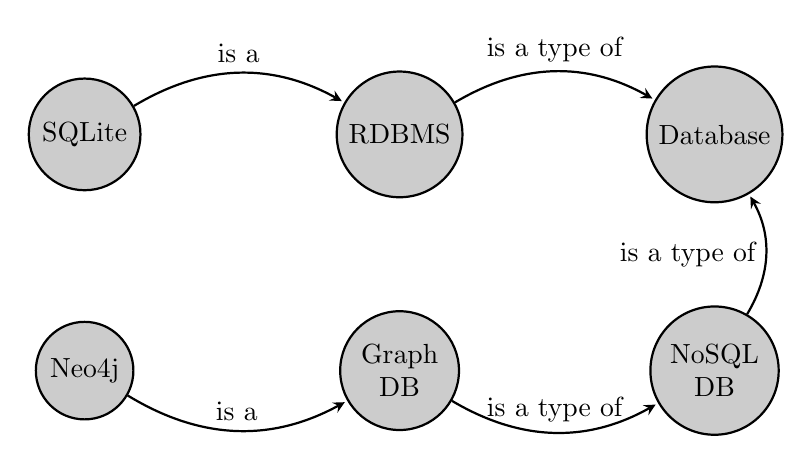
\begin{tikzpicture}[->,>=stealth,shorten >= 1 pt,auto,node distance = 3 cm,
		thick,main node/.style={circle, fill = black!20 ,draw, align = center}]
		
		\node[main node] at (0,0) (1) {Neo4j};
		\node[main node] at (4,0) (2)  {Graph\\ DB};
		\node[main node] at (8,0) (3) {NoSQL\\ DB};
		\node[main node] at (8,3) (4) {Database};
		\node[main node] at (4,3) (5) {RDBMS};
		\node[main node] at (0,3) (6) {SQLite};
		\path
		(1) edge [bend right] node {is a} (2)
		(2) edge [bend right] node {is a type of} (3)
		(3) edge [bend right] node {is a type of} (4)
		;
		\path 
		(6) edge [bend left] node {is a} (5)
		(5) edge [bend left] node {is a type of} (4)
		;
		
		\end{tikzpicture}
		\caption{Example of data stored in a graph database}
		\label{neo4eg}
	\end{figure}
	
	In this application the data being stored will be that of Facebook relationships. Graph databases are orders of magnitudes faster than a RDBMS for queries on this kind of data, such as finding extended friend networks of individuals \cite{graphdbs}.  Figure \ref{friends} shows an example of the kind of data that will be stored in the database.
	
	\begin{figure}[htbp]
		\centering
		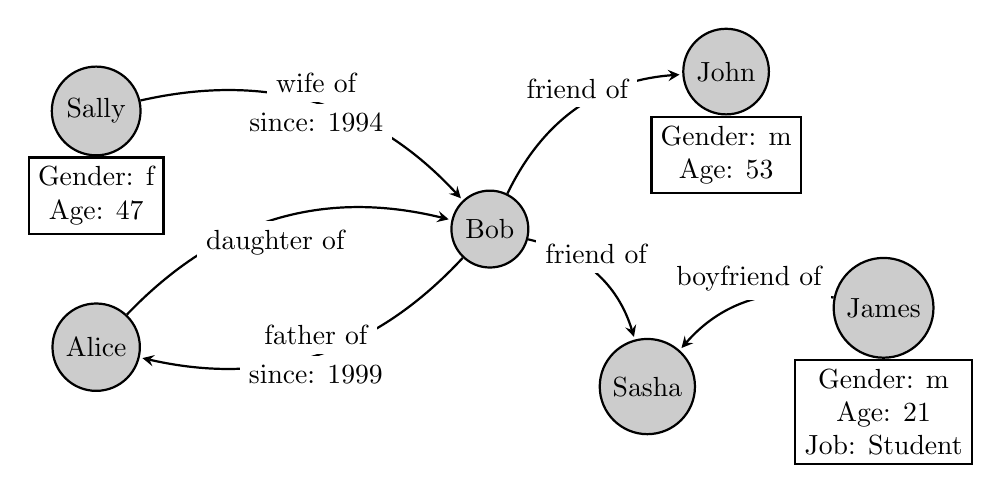
\begin{tikzpicture}[->,>=stealth,shorten >=1pt,auto,thick,main node/.style={circle,fill=black!20,draw,align=center}]
		
		\node[main node] at (-1,-0.5) (1) {Sally};
		\node[draw,rectangle, below = 0cm of 1, align=center,fill=white] (7) {Gender: f\\ Age: 47};
		\node[main node] at (7,0) (2)  {John};
		\node[draw,rectangle, below  = 0cm of 2, align=center, fill=white] (6) {Gender: m\\ Age: 53};
		\node[main node] at (4,-2) (3) {Bob};
		\node[main node] at (-1,-3.5) (4) {Alice};
		\node[main node] at (6,-4) (5) {Sasha};
		\node[main node] at (9,-3) (8) {James};
		\node[draw,rectangle, below  = 0cm of 8, align=center, fill=white] (9) {Gender: m\\ Age: 21\\ Job: Student};
		
		
		\path
		(1) edge[bend left] node[above, fill=white] {wife of} node[below,fill=white] {since: 1994} (3)
		(3) edge[bend left] node[above,fill=white] {friend of} (5)
		(3) edge[bend left] node[above,fill=white] {father of} node[below,fill=white] {since: 1999} (4)
		(3) edge[bend left] node[above,fill=white] {friend of} (2)
		(8) edge[bend right] node[above,fill=white] {boyfriend of} (5)
		(4) edge[bend left] node[below,fill=white] {daughter of} (3)
		;
		
		\end{tikzpicture}
		\caption{Example of facebook type data in a graph database}
		\label{friends}
	\end{figure}
	Note, from Figure \ref{friends}, that both the relationships as well as the entities themselves have associated data. In fact, each entity acts as a key value store. Queries can be performed to find all friends since a certain date or all friends of friends (as discussed above). These queries can be performed using Neo4j's Cypher query language or via language drivers. The language driver that will be used for this application is Py2neo.
	
	\subsection{Supporting Software}
	The Interconnected Facebook Links project is intended to be used by a Facebook user and the assumption upon which all user interfaces will be built is that the user is not technologically advanced. Therefore the final product needs to be user friendly and easy to use. The supporting software mentioned in this section describes the technologies that will be used to ensure the aforementioned user-friendliness and functionality of the product is achieved. The framework and internal structure  of the project in terms of the architecture, front-end and back-end has been described in the previous sections. This section describes the software that will be used to support these mentioned structures.
	
	In order to ensure that the end program is easy to use and looks professional, the visual design and theme needs to have a consistent, well designed layout and be visually appealing. Bootstrap is an HTML, CSS and JavaScript framework that allows this charming front-end visual design to be achieved \cite{Bootstrap}. Bootstrap provides various templates that will maintain the consistent theme throughout the final website. It also provides navigational links for the website and the template is customisable so it can be used to create the desired theme.
	
	Another technology that will support the functionally of the website is the d3.js JavaScript graphical library \cite{D3}. This library contains JavaScript code for many different visualisation graphs that can be used to visualize the data stored in the Neo4j database. Considering that the main requirement for this project is to visualise the interconnections, the 'force-directed graph' from the d3.js library will be used. As mentioned, other visualisations from the d3.js library can also be used to the further explore the database. These other visualisations include dynamic bar and line charts, geographical heat-maps and dc.js cross-filter graphs, as well as a variety of other options that may be used if they match the functionality appropriately.
	
	\subsection{Use Cases}
	A number of important use cases describing the base functionality of the product are listed and described in Table \ref{usecase}. The relationships between the use cases are shown in Figure \ref{usecased}.
	
	\begin{figure}[htbp]
		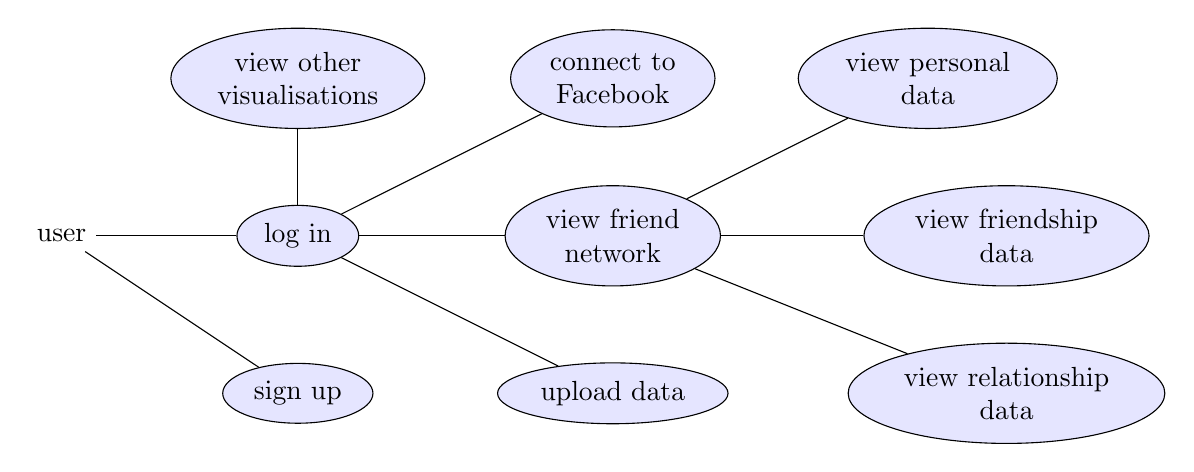
\begin{tikzpicture}[]
		
		\node at (-1,0) (user) {user};
		\node[ellipse, draw, fill = blue!10] at (2,-2) (su) {sign up};
		\node[ellipse, draw, fill = blue!10] at (2,0) (li) {log in};
		\node[ellipse, draw, fill = blue!10, align = center] at (6,2) (cf) {connect to \\ Facebook};
		\node[ellipse, draw, fill = blue!10] at (6,-2) (ud) {upload data};
		\node[ellipse, draw, fill = blue!10, align = center] at (6,0) (vf) {view friend \\ network};
		\node[ellipse, draw, fill = blue!10, align = center] at (11,0) (vfd) {view friendship \\ data};
		\node[ellipse, draw, fill = blue!10, align = center] at (11,-2) (vrd) {view relationship \\ data};
		\node[ellipse, draw, fill = blue!10, align = center] at (10,2) (vpd) {view personal \\ data};
		\node[ellipse, draw, fill = blue!10, align = center] at (2, 2) (vov) {view other \\ visualisations};
		
		\path
		(user) edge[] (su)
		(user) edge[] (li)
		(li) edge[] (cf)
		(li) edge[] (vf)
		(li) edge[] (ud)
		(vf) edge[] (vfd)
		(vf) edge[] (vrd)
		(vf) edge[] (vpd)
		(li) edge[] (vov)
		;
		
		\end{tikzpicture}
		\caption{Use case diagram}
		\label{usecased}
	\end{figure}
	
	There are a number of other use cases for the application. These would include the use of more visualisations as well as use by other types of users such as data scientists, sociologists and marketing professionals. The other visualisations were not highlighted as they do not form a part of the core functionality of the application which is to view interconnected Facebook links. The other users were not included because they do not form a part of the basic functionality in the first iterations of the application - they are not within the scope of this document. These use cases are expanded in the Appendix Section \ref{moreusecase}.
	
	\begin{table} [htbp]
		\caption{Crucial use cases for the product}
		\label{usecase}
		\centering
		\begin{tabular}{p{0.3\textwidth}|p{0.7\textwidth}}
			\hline
			\textbf{Use case} & \textbf{Description} \\ \hline
			log in & The user has to log in in order to access the various views and analytics for their data \\
			sign up & The user has to sign up to be able to log in for the first time \\
			connect to Facebook & The user can connect to their Facebook account to pull data from the Facebook API \\
			upload data & The user can manually upload their friend network data \\
			view friend network & The user views their friend network, showing friends and friends of friends \\
			view friendship data & The user views the details of the friendship links in the friend network view \\
			view relationship data & The user views the details of the relationship links in the friend network view \\
			view personal data & The user views the personal details of their friends in the friend network view \\
			view other visualisations & The user can view other visualisations of their data \\ \hline
		\end{tabular}
	\end{table}
	
	
	
	\section{The Front-End}	
	
	\subsection{Design Document} % Joe
	This section was written in accordance with the IEEE Std 1016-1987 for SDDs \cite{IEEE}. 
	
	The front-end design consists of a landing navigational web page, a friend status word chart web page and a friend network diagram web page. These web pages together represent the front-end aspect of a web application for viewing interconnected Facebook links.
	
	The section is divided into sub sections representing the different views of the design, namely the home page view, the friend network diagram view and the friend status word chart view. Each of these views represent a single interlinked web page.
	
	\subsubsection{Landing Navigational Web Page}
	The landing page was designed using a mark-up methodology for visualisation. This section describes each element of the page as well as its dependencies.
	
	The web page consists of several elements: a navigation bar, a body and a footer. The navigation bar contains links to each of the other web pages. The body contains two visual links to the other two web pages. The visual links are screen shots of the other pages which when selected navigate to the corresponding page. The footer contains copyright information.
	
	The page has the following dependencies: HTML, Bootstrap and the screen shot image files \cite{HTML, Bootstrap}. HTML was the mark-up language used for the page. Bootstrap was used for styling the page.
	
	\subsubsection{Friend Status Update Word Chart Web Page}
	The friend status word chart web page was designed using a mark-up methodology for visualisation along with some functional dependence. This section describes each element of the page, the script it uses as well as its dependencies.
		
	The web page consists of several elements: a navigation bar, a body and a description. The navigation bar contains links to each of the other web pages. The body contains the word chart visualisation. The description simply describes what is being visualised. The visualisation shows circles (each containing a common word with recent status updates). The more times a word has occurred, the larger the circles are. If hovered over the circle also reveals the exact number of times the word has appeared in recent status updates.
	
	The web page uses a code script for creating the visualisation it displays.  The general operation of the script is pictured in Figure \ref{fig:wordchart}.
	
		\begin{figure}[h]
			\centering
			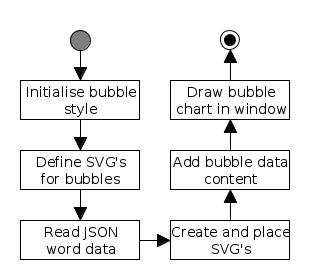
\includegraphics[scale=1]{bubbles}
			\caption{Code structure for bubble chart drawing script where SVG is Scalable Vector Graphic.} \label{fig:wordchart}
		\end{figure}

	The page has the following dependencies: HTML, Bootstrap, d3.js, Javascript and JSON formatted word data \cite{HTML, Bootstrap, D3, js, JSON}. HTML was the mark-up language used for the page. Bootstrap was used for styling the page. d3.js was used for the providing the framework to create the word chart visualisation. Javascript was used to write the script for creating the visualisation on the page. The word data was also used by the script to create the visualisation.
	
	\subsubsection{Friend Network Diagram Web Page}
	The friend network diagram web page was designed using a mark-up methodology for visualisation along with some functional dependence. This section describes each element of the page, the script it uses as well as its dependencies.

	The web page consists of several elements: a navigation bar, a body and a description. The navigation bar contains links to each of the other web pages. The body contains the friend network visualisation. The description simply describes what is being visualised. The visualisation shows profile pictures of friends in the network with lines between them representing friendship. The pictures can be dragged around the screen and stuck in place. The images also grow slightly while a user's cursor is over it.
	
	The web page uses a code script for creating the visualisation it displays.  The general operation of the script is pictured in Figure \ref{fig:networkdiagram}.
	
		\begin{figure}[h]
			\centering
			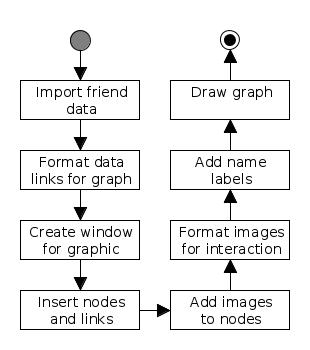
\includegraphics[scale=1]{network}
			\caption{Code structure for friend network drawing script.} \label{fig:networkdiagram}
		\end{figure}
		
	The page has the following dependencies: HTML, Bootstrap, d3.js, Javascript and JSON formatted word data \cite{HTML, Bootstrap, D3, js, JSON}. HTML was the mark-up language used for the page. Bootstrap was used for styling the page. d3.js was used for the providing the framework to create the word chart visualisation. Javascript was used to write the script for creating the visualisation on the page. The word data was also used by the script to create the visualisation.

	The section is divided into sub sections representing the different views of the design, namely the home page view, the friend network diagram view and the friend status word chart view.
	\begin{figure}[h]
		\centering
		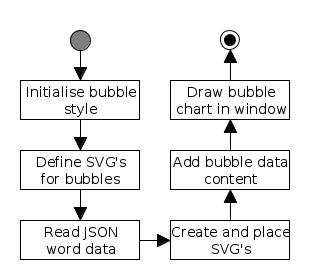
\includegraphics[scale=1]{bubbles}
		\caption{Code structure for bubble chart drawing script.}
	\end{figure}
	
	\begin{figure}[h]
		\centering
		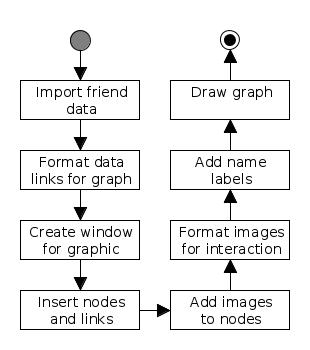
\includegraphics[scale=1]{network}
		\caption{Code structure for friend network drawing script.}
	\end{figure}
	
	\subsection{Implementation} % Nathan
	
	\subsubsection{Introduction}
	The implementation of the front-end user interface formed the simpler aspect of the project. The front-end was created with HTML, using Bootstrap styling to create a desirable look and feel. The visualisations themselves, which were created using d3.js, were called in the HTML as script elements through Django's \textit{static files} functionality. 
	In order to provide developers with the ability to add new functionality easily and to ensure scalability, a separate module exists for each visualisation that the software presents to end-users. This means that to add a new visualisation, three separate steps need to occur:
	
	\begin{enumerate}
		\item Create an HTML page to present the visualisation.
		\item Implement the script that produces the visualistion.
		\item Add the new HTML page to the index, allow users to navigate between visualisations.
	\end{enumerate}
	
	\subsubsection{Implementing HTML pages with Django}
	Django refers to HTML pages as \textit{templates}. The initial implementation of the web pages consisted of coding a page using HTML and Bootstrap, and testing that the inserted scripts worked correctly in producing the visualisations. Once the scripts had been tested, the pages were integrated with Django. Instead of referring to the normal Bootstrap files, the page referred to the Bootstrap file found within Django's static files environment.
	
	Static files are loaded into the HTML page as follows:
	\begin{lstlisting}

	\end{lstlisting}
	
	To direct the HTML page to the Bootstrap styling file, the following link is called:
		\begin{lstlisting}
<link rel="stylesheet" href="">
		\end{lstlisting}
	To direct the HTML page to the d3.js functionality, the following script is called:
		\begin{lstlisting}
<link rel="stylesheet" href="">
		\end{lstlisting}
		
	Data for the friend network and for the word bubble chart is accepted in a JSON format. It is then filtered in the scripts and used to create the visualisations. Both visualisations were created using SVG  graphics, which is beneficial due to its interactive nature and powerful ability to customise. Visualisations are created dynamically and on demand, and so SVG graphics are perfectly suited to the context of the project. A major advantage of using these graphics is that they are relatively small and so users will not have to wait long to receive their visualisations \cite{SVG}.
	
	\subsubsection{Friend Network}
	The friend network was implemented using the d3.js force directed graph. To create the graph, explicit parameters were defined in the script to control the size of the graph, setting the width at 960px, the height at 500px and the radius of the  nodes in the graph to 6px. The HTML code imports the data through back-end functionality to create the friend network. 
	
	The script accepts graph data with two concepts: "nodes" and "links". The node data is used to create the nodes on the graph representing the Facebook friends of the current user. Each node has a name and a group assigned to it. The link data maps nodes to each other, describing their relationship and assigning a value to the link between the nodes. This mapping is done by defining a link as the relationship between a source node and a target node.
	
	\subsubsection{Word Bubble Chart}
	The word bubble chart was implemented using the d3.js pack layout. The d3.js pack layout allows developers to represent elements as bubbles, and the size of the bubble is determined by the frequency (also known as the size attribute) of the elements. The word bubble chart was implemented with a flattened hierarchy, meaning that there is only one level of bubbles as in figure \ref{fig:bubblechart}, as opposed to "bubble charts within bubble charts," shown in \ref{fig:packlayout}.
	
  	The script accepts graph data with two attributes: "name" and "size". Each element in the JSON file gets its own bubble. The radius of the bubble is determined by each element's associated size attribute.
  	
   \begin{figure}
   	\centering
   	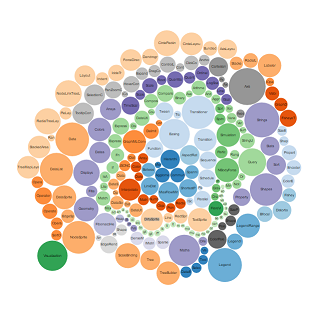
\includegraphics[scale=1]{bubblechart.PNG}
   	\caption{Bubble Chart with a flattened hierarchy} \label{fig:bubblechart}
   \end{figure}
   
   \begin{figure}
   	\centering
   	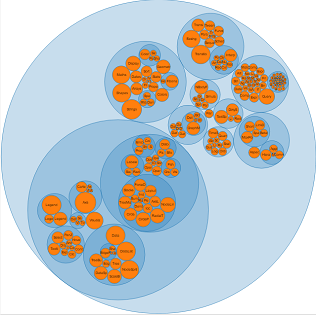
\includegraphics[scale=1]{packlayout.PNG}
   	\caption{Pack Layout, showing hierarchical composition} \label{fig:packlayout}
   \end{figure}
   
   \subsubsection{Front-End Testing}
   
   In order to ensure implementation occurred correctly, the following testing following implementation: 
   
   General testing involved ensuring that the project workflow ran smoothly. This meant following all existing links and testing that they actually worked, in other words, redirecting users to the correct pages.
   
   The friend network graph page was tested first by using dummy data to ensure that the graph behaved as expected. The graph's border, node characteristics and interaction capabilities was constantly adjusted until they were considered satisfactory. After this the network graph was tested with real data from the neo4j database to ensure integration worked as expected. All of these tests were successful.
   
   Testing of the friend status update word analysing bubble chart page involved using various sets of dummy data to see how the bubble chart changed when the size and content of the data set changed.
   
	
	\section{The Back-End}
	
	\subsection{Design Document} % Joe
	This section was written in accordance with the IEEE Std 1016-1987 for SDDs \cite{IEEE}. 
	
	The back-end design consists of a graphical database system containing supporting functionality for making friend network queries as well as a web application framework. Both views were designed using a functional methodology. The particular functionalities of the design are documented below. These views together represent the back-end aspect of a web application for viewing interconnected Facebook links.
	
	The section is divided into sub sections representing the different views of the design, namely the database view and the web application framework view.
	
	\subsubsection{The Web Application Framework}
	This section will discuss the functions, dependencies and details of the web application framework. The general operation of the system is shown in Figure \ref{fig:django}.
	
	\begin{figure}[h] 
		\centering
		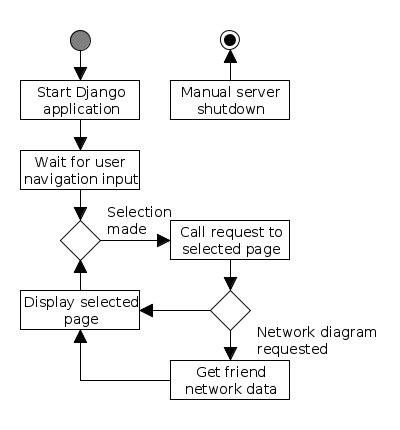
\includegraphics[scale=1]{djangostruc}
		\caption{Code structure for running of web application and processing user input.} \label{fig:django}
	\end{figure}
	
	The following functions were used in the web application framework: \texttt{home()}, \texttt{friendNetwork()} and \texttt{wordChart()}. These functions refer to the different pages served by the web application. Each of these functions simply return the file path to the requested page which is the input to each function.
	
	The \texttt{friendNetwork()} function, however, also calls a database supporting function to retrieve data which the page supported by the \texttt{friendNetwork()} function requires. The function not only returns the file path but also the content for the page to use.
	
	The web application framework has the following dependencies: Django web framework, Apache HTTP server, mod\_wsgi, Python  and the page documents \cite{django, apache, wsgi}. Django was the framework used for integrating the source code used in the web application. Apache was the HTTP server used to host the web application. mod\_wsgi integrates the Django framework and the Apache server. Python was the programming language used by the framework. The page documents were stored within the Django framework and were required by the functions described above. 
	
	Several other details of the web framework are important. Firstly, the web application file system contains all of the dependencies of the functions mentioned as well as their supporting functions. Secondly, the file system also contains several configuration files specific to Django. Finally, several other scripts are required to run to start the server and web application - these are standardly available with the dependencies used.
	
	\subsubsection{The Graph Database}
	This section will discuss the functions, dependencies and details of the the graph database. The general operation of the supporting functions of the system is shown in Figure \ref{fig:db}.
	
	\begin{figure} [htb]
		\centering
		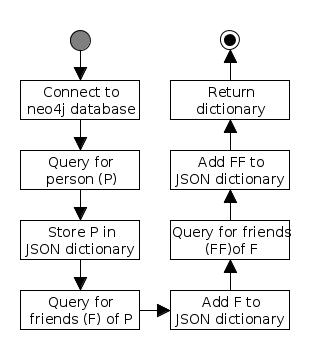
\includegraphics[scale=1]{neo4jdb}
		\caption{Code structure for fetching friends of friends network from neo4j DB.} \label{fig:db}
	\end{figure}
	
	The following functions were used to support the graphical database: \texttt{getPerson()}, \texttt{getFriendNetwork()} and \texttt{getFoFNetwork()}. These functions each take as inputs the name and surname of the person being queried and return a dictionary containing the query results. 
	
	The \texttt{getPerson()} function uses the name and surname input to query the database for the requested person. The function returns a dictionary containing the person in a node.
	
	The \texttt{getFriendNetwork()} function uses the name and surname input to query the database for the requested person and the person's friends as well as the links between them. This function makes use of the \texttt{getPerson()} function. The function returns a dictionary containing all of the queried persons in nodes and the relationships between them in links.
	
	The \texttt{getFoFNetwork()} function uses the name and surname input to query the database for the requested person, the person's friends and the friends of the person's friends as well as the links between them. This function makes use of the \texttt{getFriendNetwork()} function. The function returns a dictionary containing all of the queried persons in nodes and the relationships between them in links.
	
	The graphical database has the following dependencies: Neo4j, Py2neo and JSON \cite{neo4j, py2neo, JSON}. Neo4j was the graphical database used in the software. Py2neo was the Python API which was used in order to enable use of the database by the Python programming language. The web framework required use of Python. The dictionaries returned by the functions mentioned above were in JSON format.
	
	Two other details of the database are important. Firstly, the fields in the dictionaries returned by the above functions were nodes and links where each node and link had sub-fields. An example of their format is shown in Listing \ref{list:dbjson}. Secondly, the database requires an initialisation and migration to start it up. Standard code is provided for these functionalities.
	
	\begin{lstlisting}[caption=test,captionpos=b,label=list:dbjson]
	{
	    "links": [
	        {
	            "level": "None", 
	            "since": "2014", 
	            "source": 248, 
	            "target": 247, 
	            "type": "FRIENDS_WITH"
	        }, 
	        {
	            "level": "dating", 
	            "since": "2015", 
	            "source": 248, 
	            "target": 252, 
	            "type": "IN_RELATIONSHIP_WITH"
	        }, 
	        {
	            "level": "None", 
	            "since": "2013", 
	            "source": 248, 
	            "target": 249, 
	            "type": "FRIENDS_WITH"
	        }
	    ], 
	    "nodes": [
	        {
	            "age": null, 
	            "id": 247, 
	            "img_url": "", 
	            "name": "Paul", 
	            "occupation": "None", 
	            "surname": "Cresswell"
	        }, 
	        {
	            "age": 21, 
	            "id": 248, 
	            "img_url": "", 
	            "name": "James", 
	            "occupation": "Student", 
	            "surname": "Allingham"
	        }, 
	        {
	            "age": 21, 
	            "id": 249, 
	            "img_url": "", 
	            "name": "Julian", 
	            "occupation": "Data Scientist", 
	            "surname": "Zeegers"
	        }
	    ]
	}

	\end{lstlisting} 
	
	\subsection{Implementation} % Nathan
	
	\section{The Sprint Planning}
	The Scrum process is an agile approach to projects (particularly software development projects) that encourages incremental progress, teamwork, collaboration with clients and allows for sudden requirement changes \cite{Cohn}. This process is comprised of short project sprints (typically 30 days) with each sprint focusing on the succeeding project requirements. This incremental approach requires functionally of aspects of the project after each sprint. This section discusses the sprint planning progress and the Scrum approach taken for the Tracking Interconnected Facebook Links project. Figure \ref{fig:scrum} illustrates the Scrum process and the labeled numbered sections 1, 2 and 3 are discussed in Sections  \ref{scrumback} ,  \ref{sprintback} and  \ref{retro} respectively.
	
\begin{center}
	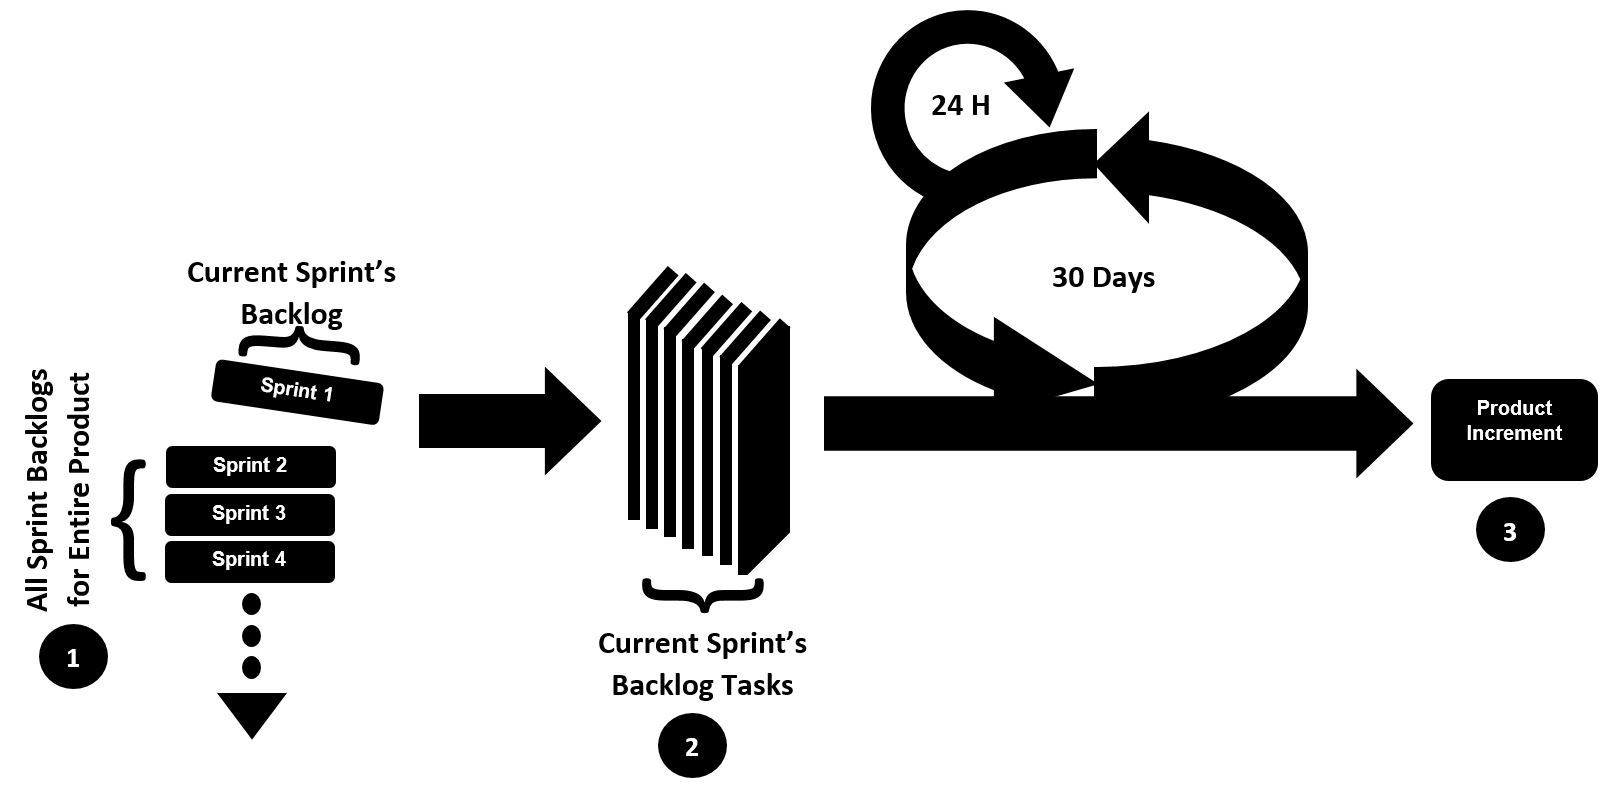
\includegraphics[width=\textwidth]{scrum}
	\captionof{figure}{Diagram of the entire Scrum Process adapted from \cite{Haunts}} \label{fig:scrum}
\end{center}
		
		

	
	\subsection{The Scrum Backlog } \label{scrumback}
	The Scrum backlog (labeled "1" in Figure \ref{fig:scrum}) is a backlog that contains all the tasks for the entire project that are required to be completed. The formation of the Scrum backlog is complied by the Scrum team and the product owner to ensure that the defined tasks are closely in line with the requirements for the project. The Scrum team for Tracking Facebook Interconnected Links project is comprised of four software developers with two members forming the back-end team and two members forming the front-end team. The backlog comprises of the various task definitions, a time estimation of each task and the task's priority. The Scrum backlog is made at the beginning of the project during the planning stage. This backlog is flexible as tasks can be added, changed and re-prioritized by the product owner, the scrum team or other stakeholders during the project development. The Scrum Product Backlog for the Tracking Facebook Interconnected Links is shown in Table \ref{backlog} which includes all the tasks, the estimated time and priority.     
	
	\begin{longtable}{|>{\centering\arraybackslash}p{1cm}|p{8cm}|>{\centering\arraybackslash}p{1.5cm}|>{\centering\arraybackslash}p{1.5cm}|}
		\caption{The Scrum Product Backlog\label{backlog}}\\
		\hline 
		ID & \centering  Task Description  &  Estimate (days) & Priority   \\
		\hline
		2 	& Start a Django project and change to required settings	& 2 & 1\\
		\hline
		1 & Create neo4j database 	&  2 & 2 \\
		\hline 		
		3	& Make an HTML landing page view. This should also be a template for the other views and therefore must make use of a bootstrap theme and have navigational links. 	& 1 & 3\\
		\hline 
		4	& Source Facebook user data and load it onto the database. Obtain the required permissions to access this data. The data must be stored in a logical and structured fashion in order to ensure the data can be accessed as required. 	& 3 & 4\\
		\hline
		10	& Write Python scripts and functions that return data required by the different views in a correct format (i.e. JSON, CSV, TSV etc.) by using database queries 	& 3 & 5\\ 
		\hline
		5	& Create a view that contains a d3.js "Force-diagram" that is used to visualize a friend network diagram that is interactively used by the end user. 	& 5 & 6\\
		\hline 
		6	& Create a view that contains a d3.js "Word bubble chart" that visualizes the popularity of words used by Facebook friends of the end user in their Facebook status.	& 4 & 7\\
		\hline 
		7	& Set-up an Apache server on a server host computer and host the Django project that contains the various views. 	& 2 & 8 \\
		\hline 
		8	& Integrate the first phase systems required for the first sprint. This includes linking all the views to their URLs in the Django project framework, connect the neo4j database to the Django project, ensure that the views are able to pull required data from the database and that the Apache server successful hosts the project.  	& 3 & 9\\
		\hline 
		9	& Do various software tests to ensure the integration is successful. These tests include testing the database queries return expected data, tests that the graphs in the views visualize the correct information and test that the Apache server host all the URLs  	& 3 & 10\\
		\hline  
		11	& Register for a domain name and host the Apache server to that domain in order to allow the project to be accessed on the Internet.	& 2 & 11\\
		\hline
		15	& Addition Python scripts and functions for the new views	& 3 & 12\\
		\hline	
		12	& Create a view that makes use of a d3.js library called crossfilter.js. This view must contain charts that visualize the user's various Facebook friend relationship data using bar charts, line charts and pie chart. Each chart in this view must filter the other charts &  3 & 13\\
		\hline
		13	& Create a view that illustrates the degrees of separation between Facebook users. This view must take two names as an input of calculate the degree of separation between them.	&  4 & 14\\
		\hline
		14	& View that can user the friend relationships to plan global trips for the user	& 6  & 15\\
		\hline
		16	& Write a Python script that implements machine learning that the user can use to predict potential friend pairings.    	& 10 & 16\\
		\hline
		17	& Preform addition tests on the new views created.	& 2 & 17\\
		\hline
		18	& Create a login interface where a user can create an account and login into the web application. An additional table to the database must be added to store these details.	& 5 & 18\\
		\hline
		19	& Make a Facebook API for automatically pulling user information from the Facebook website. This should allow all the view to be updated with the latest data	& 4 & 19\\
		\hline
		20	& Implement the HTTPS protocol on the server to ensure that the web application is more secure	& 3 & 20\\
		\hline
		21	& Create automated tests that continuously tests the software to ensure that it is always working as required 	& 4 & 21\\
		\hline
		& \textbf{Total }	& 74 Days & \\
		\hline 	
	\end{longtable}
	
	The Scrum backlog shown in Table \ref{backlog} was complied at the beginning of the project by the Scrum team and product owner during the Scrum planning session. All tasks that are deemed necessary for the entire project are recorded in the backlog. As mentioned, this backlog is adjustable as there is a possibility that new tasks may arise during the project. Smaller meetings with th product owner and Scrum team will be conducted when the backlog needs to be adjusted. During the Scrum planning meetings, the logistics of the entire project in terms of the working environment and communication forums are also discussed in this meeting and is described in the next section.
	
	\subsection{The Scrum Logistics} \label{log}
	The project logistics and the formation of the working environment are discussed the Scrum planning meeting. Firstly, the created project's software needs a central submission repository where all the project's software can be accessed. A Github repository is created and each member of the Scrum team are invited to join this repository and are given access to this repository. This repository is also used for the software version control and a is technology to allows collaborative software development.
	

	
	\begin{center}
		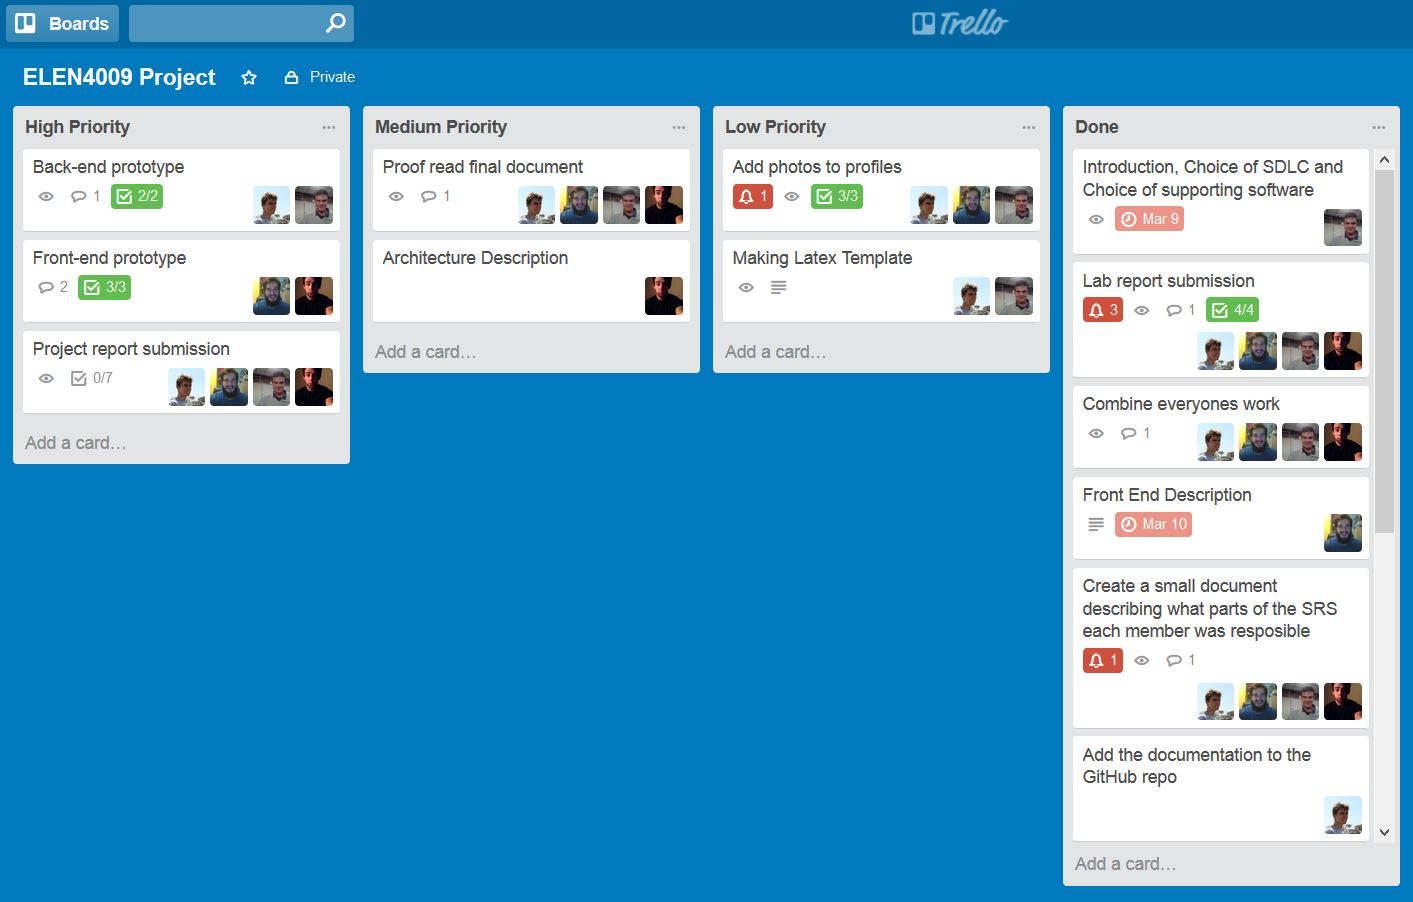
\includegraphics[width=\textwidth]{trello}
		\captionof{figure}{Screen shot of the Trello web application taken from \cite{trello}} \label{fig:trello}
	\end{center}
	
	In terms of communication, there are various platforms used to organize, ask questions or give comments with regards to the project. These platforms include Github, Trello and Slack. Github is used as a form of communication as the commit messages are used to keep track of completed tasks. Another platform called Trello is also used to keep track of progress and it also servers as a task organisation tool \cite{trello}. A screen shot of the Trello web application is shown in Figure \ref{fig:trello}. This application has prioritized "boards" that are ranged in three levels of priorities; namely high, medium and low. The Scrum master adds each task in the form of a "card" to a prioritized board with information associated with the task such as the member or members responsible for the task, the deadline and a task check list. Once a task card is completed, the team member who completed the task moves the task to the done board. This web application can can be downloaded as a mobile application by each Scrum team member and is useful for the Scrum master and team members to keep track of project progress. Figure \ref{fig:trello} show a screen shot of the Trello web application and shows an example of the "boards" and "cards" using for the project.
	

	\begin{center}
		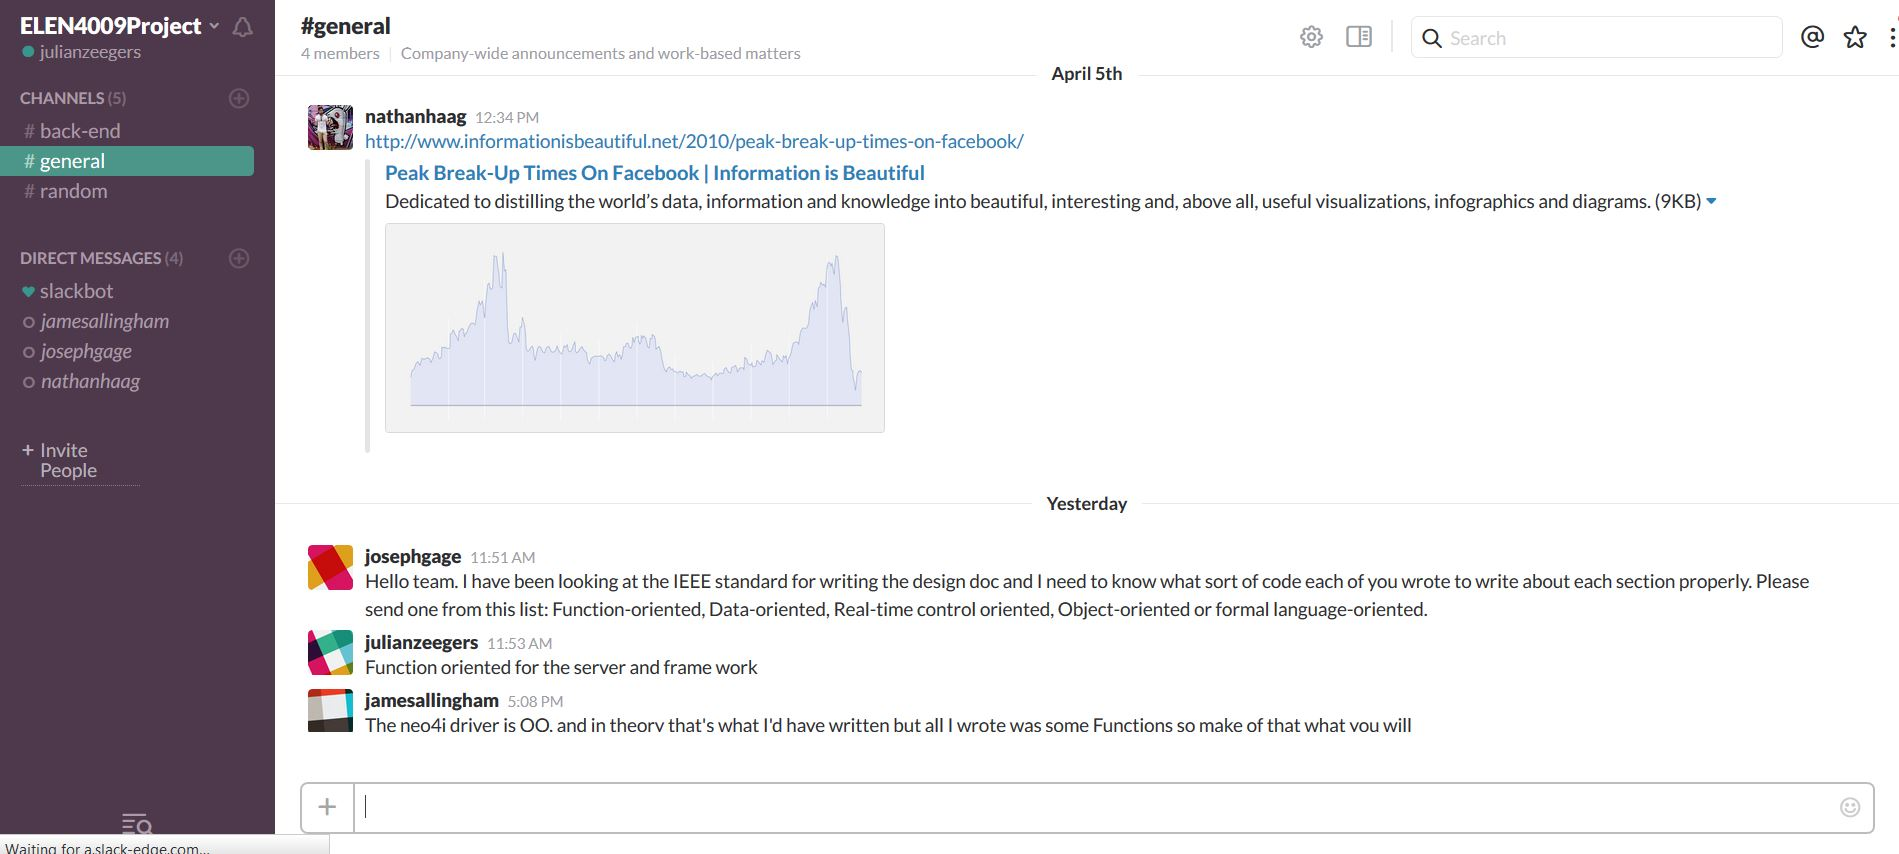
\includegraphics[width=\textwidth]{slick}
		\captionof{figure}{Screen shot of the Slack messaging application taken from \cite{slack}} \label{fig:slack}
	\end{center}
	
	Another communication forum used for this project is called Slack and this messaging platform is used by the Scrum team members to ask questions and post comments about the project \cite{slack}. This platform is different from other messaging platforms as users can also post code and get help from the other members for certain coding problems. Slack is also used to organize project events such as Scrum meetings, demonstration events and communicate deadlines. A screen shot of the Slack messaging platform is shown in Figure \ref{fig:slack} and it also shows an example of a typical project conversation.
	
	
	
	These technologies and communication tools are used extensively during each sprint of the Scrum to ensure the sprint runs smoothly. The first sprint for the Tracking Facebook Interconnected Links project is discussed in the next section. 
	
	
	\subsection{The Sprint Backlog } \label{sprintback}
	A sprint is an iteration of the project's product and it is a stage within in the Scrum progress. A sprint in typically two to four weeks long and it should produce a shippable increment of the product at the end of the sprint. A sprint is comprised of tasks defined in a sprint backlog and is labeled "2" in Figure \ref{fig:scrum}. The sprint backlog is made up of certain tasks already defined in the Scrum product backlog (discussed in Section \ref{scrumback}) and these task are the most prioritized task remaining within the product backlog. 
	
	The first sprint for the Tracking Facebook Interconnected Links project is planned in a sprint planning meeting conducted between the Scrum members. This meeting is run for about 6 hours because the sprint is planned to run for about 4 weeks. During this meeting a sprint product backlog is drawn up and is shown in Table \ref{sprintbacklog}. As shown in Table \ref{sprintbacklog}, a short description of each task is defined as while as the duration of each task. It also shows the number of days in each week of the sprint each task should be worked on for. The overall sprint goals are defined for the sprint in this meeting which outline the expectations of the sprint's end product. For this first sprint, the following sprint goals are set out:
	
	\begin{itemize}
		\item Create a project prototype that includes one landing page and two functional views.
		\item Create and populate the database.
		\item Set-up the system's architecture such as setting up the framework and server. 
	\end{itemize}
	
	
	\begin{longtable}[h!]{|>{\centering\arraybackslash}p{0.5cm}|p{6.5cm}|>{\centering\arraybackslash}p{1.1cm}|>{\centering\arraybackslash}p{1.1cm}|>{\centering\arraybackslash}p{1.1cm}|>{\centering\arraybackslash}p{1cm}|}\caption{The Sprint Product Backlog\label{sprintbacklog}}\\
		\hline
		\multicolumn{2}{|c|}{}  &  \multicolumn{4}{c|}{Days Task Worked on per Week}  \\
		\hline
		ID & \centering Short Task Description & Week 1 & Week 2 & Week 3 & Week 4   \\
		\hline
		2 	& Start a Django project	& 2 &   & &  \\
		\hline
		1 & Create neo4j database 	&  2 &   & & \\
		\hline 	
		3	& Make an HTML landing page view with a bootstrap theme and navigational links. 	& 1 &  & & \\
		\hline 
		4	& Source Facebook user data and load it onto the database & 2 & 1  &  & \\
		\hline
		10	& Write Python scripts and functions that return data required in a correct format &  & 2  & 1 & \\ 
		\hline
		5	& Create a view that contains a d3.js "Force-diagram" that is used to visualize a friend network diagram	&  & 2  & 2 & 1 \\
		\hline 
		6	& Create a view that contains a d3.js "Word bubble chart" that visualizes the popularity of words used in status	&  & 1 & 2 & 1 \\
		\hline 
		7	& Set-up an Apache server that host the Django project &  &   & 2 & \\
		\hline 
		8	& Integrate the first phase systems.	&  &  & 2 & 1\\
		\hline 
		9	& Do software testing  	&  & & & 3 \\
		\hline 	
		
		
	\end{longtable}
	
	Each task is also allocated to a Scrum team member during this sprint planning meeting. The team members choose the tasks that they would like to do with the front-end and back-end team members choosing their respective tasks. Once the tasks are scheduled to the team, a new Trello board is created with the new task allocations (as discussed in Section \ref{log}). The tasks described in Table \ref{sprintbacklog} are subjected to change, however these changes must not change the sprint's goals that were outlined. There were minutes that were taken for the Sprint planning meeting and these minutes can be found in Appendix B. In Appendix B, some project roles were simulated such as the Product Owner, Project Administrator, the Scrum Master and Marketing Manager in order add authenticity to the meeting that took place.
	
	\subsection{The Daily Scrum Meetings}
	
	 Once the sprint begins, there is a daily Scrum meeting that occurs in the morning of each working day. During this meeting, each Scrum team member is given the opportunity for report on their daily progress. Each member is also required to talk about the following items:
	
	\begin{itemize}
		\item The tasks that they completed since the previous meeting
		\item The tasks that they plan to work on after the current meeting
		\item Any project challenges that they are currently struggling with 
	\end{itemize}
	
	These daily Scrum meetings are meant to be relatively short (typically 15 minutes) and the objective of these meetings is to provide a platform for the Scrum team to keep track of progress. These meetings also allow for the members to obtain help or get ideas on how to solve small problems and can be used to communicate small project plan changes. 
	
	\subsection{Managing The Sprint Process}
	The sprint process of the project is an effective methodology that allows rapid software development that can be flexible in terms of the requirements. However, the fast paced nature the sprint can be chaotic and disorganized and it is therefore very important to mange the project well. An organized, disciplined Project Manager (can also be the Scrum Master) must be appointed to ensure the project is well organized. Various project managing tools must be utilized in order to ensure the sprint achieves the set out sprint goals. Tools that have already been mentioned include conducting daily meetings and using the communication platforms effectively to maintain project progress. Another project managing tool that can be used is a Gantt chart. A Gantt shows the various tasks defined in the sprint backlog on a time-line. It illustrates to the Project Manager when certain tasks must be completed by, which team members are responsible for each task and also shows the critical path. The critical path are tasks in which the deadlines are crucial as delays with these tasks could cause delays for the entire sprint. The Gantt chart for the first sprint is drawn up and is shown in Figure \ref{fig:gantt}
	
	\begin{center}
		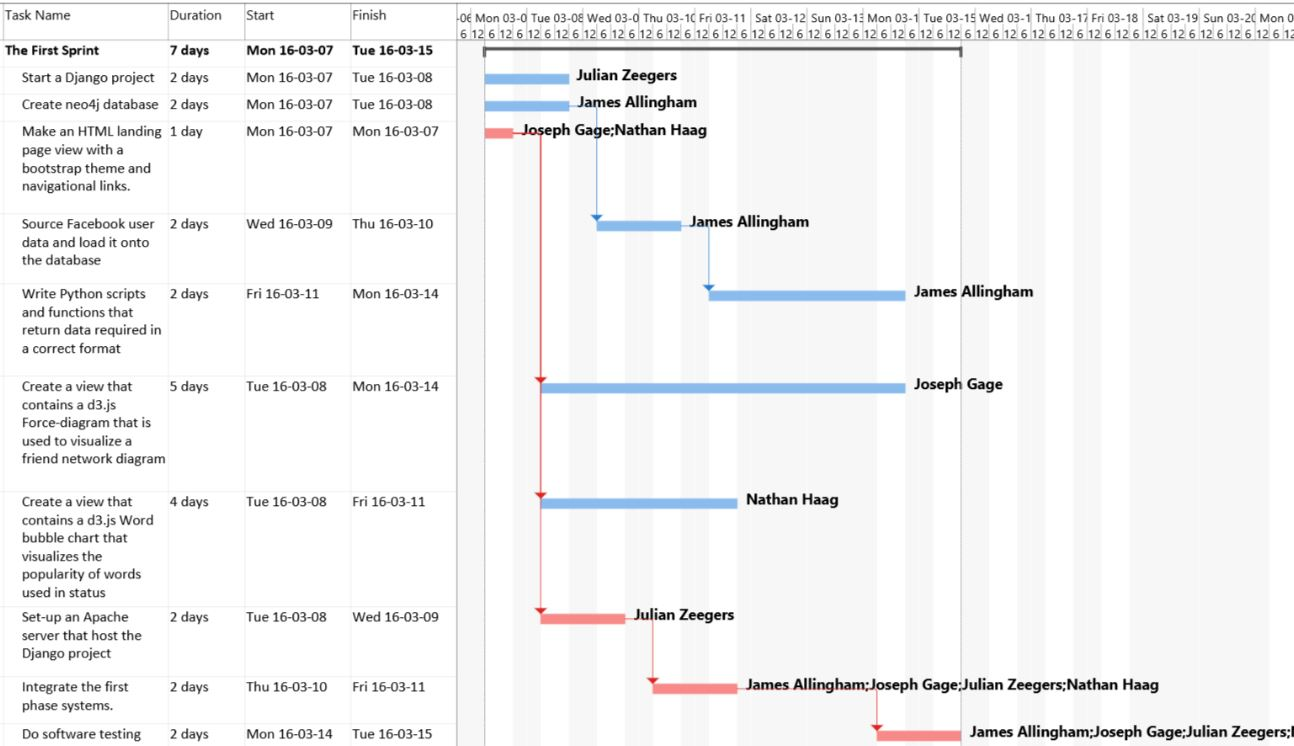
\includegraphics[width=\textwidth]{gantt}
		\captionof{figure}{Screen shot of Gantt Chart} \label{fig:gantt}
	\end{center}
	

	\section{Sprint Retrospective} \label{retro}
	Once a sprint is completed, there is a meeting conducted in which the sprint is reviewed and this meeting is called the Sprint Retrospective Meeting. During this meeting, many items related to the sprint are discussed which includes the successful goals achieved, the goals that were not achieved, the challenges that were face and how well the Scrum team worked together. As mentioned, at the end of a sprint, a shippable product must be created that achieves the basic sprint goals (as shown by the label "3" in Figure \ref{fig:scrum}). The sprint product is reviewed in this meeting and the Scrum team members are also given an opportunity to express there opinion. This section discusses all these aspects of the sprint retrospective.
	
	\subsection{The Goals Achieved and Positive Outcomes}
	After the first sprint, a shippable prototype of the Tracking Facebook Interconnected Links project was produced by the Scrum team. The following goals were successfully achieved:
	
	\begin{itemize}
		\item A web application with a landing page and two functional views was created.
		\item The data for the views is stored in a neo4j graph database and the required data is pulled for the database using Cypher queries and Python functions.
		\item The web application is hosted on an Apache web server.
	\end{itemize}
	
	The sprint's end product is functional and a detailed user guide document was written up which instructs the user on how to use the product. All the initial system environments were successful set-up such as the database, server, Django project and bootstrap theme which will not need to be done again in future sprints. This allows the next sprint to be able to focus more on creating more views and increasing functionally. 
	
	In terms of the working environment, the sprint process was relatively well organized which allowed these goals to be achieved. The Scrum team made effective use of the Trello and Github platforms. In particular, the Trello board was updated regularly with completed and new tasks which allowed the team to keep track of progress. The Github respiratory was also used effectively for integrating and storing the various tasks.
	
	The sprint was also well documented which will make progressing in the next sprint easier. A fully detailed Software Requirement Specification was created and can be used in future sprints to ensure that the progress is in line with what is required. A design document, implementation document and user guide was written which will also help with future project progression. 
	
	\subsection{The Negative Outcomes} \label{neg}
	Although the first sprint achieved the goals that were set up for the sprint, a few negative outcomes occurred during the sprint. It is important to identify these negative aspects in order to improve them for the next sprint. These negative outcomes include the following:
	
	\begin{itemize}
		\item The overall layout, design and chosen bootstrap theme used for the web application lacks attractiveness.
		\item There is not enough data in the database. Although the sprint's end product is only a prototype, much more data is required to make the graphs for each view more functional.
		\item The created views are not as interactive as they should be. More functionality must be added to them.
		\item Did not make full use of the Django project as the "models" aspect of Django was not utilized. 
	\end{itemize}
	
	One negative aspect of the working environment was a lack of communication between the Scrum members at times. The Slack messaging platform was not fully utilized by the members to communicate. Often communication about challenges and problems faced by a member was dealt with in person with only one or two other members present. This meant that many times the entire team were not involved in that communication and therefore input and insight from the missing members could not happen. 
	
	Another problem faced was that the tasks were sometimes completed after the planned deadlines. This caused a slight build up of work towards the end of the sprint and final integration tasks were rushed. These mentioned negative outcomes need to be considered when planning the next sprint as this will improve the overall final project product.
	
	\subsection{The Sprint Retrospective Meeting Feedback}
	The sprint retrospective meeting gives the scrum team an opportunity to reflect on the previous sprint and and serves as an opportunity for team members to give their own input on how to improve for the next sprint. Table \ref{feedback} shows the feedback given by each member during this meeting.
	
	\begin{table}[h!]
		\caption{The Sprint Retrospective Meeting Feedback\label{feedback}}
		\small
		\begin{tabular}{|>{\centering\arraybackslash}p{1.8cm}|p{3.4cm}|p{3.4cm}|p{3.4cm}|}
			\hline
			\multicolumn{1}{|c|}{}  &  \multicolumn{3}{c|}{Feedback Questions}  \\
			\hline
			Member's Name & What went well during the last sprint? & What did not go well during the last sprint? & How can the team improve for the next sprint? \\
			\hline
			James Allingham & The team communicated well and the work was all completed on time. & The deadline for the prototype was very stressful as it was almost missed. & Work should be better integrated from the start to prevent last minute integration problems. \\
			\hline
			Joseph Gage & & & \\
			\hline
			Nathan Haag & & & \\
			\hline
			Julian Zeegers & Each member of the team knew their respective responsibility and the Trello web application work well to ensure that was the case. & There was not a lot of time left for integrating the components and the integration was therefore unnecessarily stressful.   & A better estimation for the time each task takes is required. A better visual design of the web application must be implemented.\\
			\hline
			
			
		\end{tabular}
	\end{table}
	
	
	\subsection{The Improvements For the Next Sprint}
	One of the main purposes of the sprint retrospective meeting is to highlight improvements that can be made for the next sprint and suggest plans on how to implement these improvements. The negative outcomes mentioned in Section \ref{neg} must be improved and the following are suggestions that should improve them:
	
	\begin{itemize}
		\item The design and  layout can be improved by using a better bootstrap template. It is suggested that the "Dashboard" template should be used.
		\item In order to obtain more Facebook data, the database should use a Facebook API to continuously pull data from the Facebook site. 
		\item Hosting the Apache server on a dedicated host computer server.
	\end{itemize}

	During the next sprint meetings, better task time estimation must be made, especially tasks that involve integrating the project components. The use of the Slack messaging platform must also be encouraged to allow the entire team the opportunity to help fix problems. Although the first sprint has these mentioned improvements that must be implemented, the outcome of the first sprint was successful and it has produced a good software development foundation for the future increments of the project.


	\section{Conclusion}

	The requirements, design, implementation and testing of a two-tier web-based application for visualising interconnected Facebook links has been presented. The group work aspects of the project, including SLDC as tools for communication and organisation, have been discussed. The prototype application showed that the selected technologies and tools are capable of delivering the required features and specifications. Future work for the project as well as improvements in the performance of the development team have been suggested.

	
	\begin{thebibliography}{1}
		\bibitem{IEEE} IEEE Standards Board. \emph{IEEE Guide to Software Design Descriptions}. IEEE, New York, 25 May 1993.
		
		\bibitem{fb} Statista. \url {http://www.statista.com/statistics/264810/number-of-monthly-active-facebook-users-worldwide/}. Last accessed 18 February 2016. 
		
		\bibitem{pmbok} Project Management Institute. \emph{A Guide to the Project Management Body of Knowledge (PMBOK Guide)}. Newtown Square, Pa: Project Management Institute, 2004. ch 13. p 390.
		
		\bibitem{Kinsey} H. van Vliet, \emph{Software Engineering: Principles and Practice} Wiley, 2007.
		
		\bibitem{twotieradvantage} N. Liyanage. \emph{Client/Server Architecture: Advantages and Disadvantages of the architectures}. 2013. \url{http://clientserverarch.blogspot.co.za/2013/03/advantages-and-disadvantages-of.html} Last accessed: 9 March 2016
		
		\bibitem{beginningsofteng} R. Stephens, Beginning Software Engineering, 1st ed. Indianapolis: John Wiley And Sons, Inc, 2015, pp. 94-95.
		
		\bibitem{Bootstrap}  \emph{Get Bootstrap - 3.3.6} \url{www.getbootstrap.com} Last accessed: 9 March 2016.
		
		\bibitem{D3}  \emph{d3.js - Data Driven Documents} \url{www.d3.com} Last accessed: 9 March 2016.
		
		\bibitem{SVG}  \emph{The Advantages of using SVG} \url{http://www.todaysoftmag.com/article/1067/the-advantages-of-using-svg-scalable-vector-graphics} Last accessed: 10 March 2016.
		
		\bibitem{django} Django Software Foundation. \emph{Django Overview}. \url{https://www.djangoproject.com/start/overview/}. 2016. Last accessed: 9 March 2016. 
		
		\bibitem{djangobook} Adrian Holovaty, Jacob Kaplan-Moss, et al. \emph{The Django Book}. \url{http://www.djangobook.com/en/2.0/index.html#}. Ch 3. Last accessed: 9 March 2016.
		
		\bibitem{djangoApache} Django Software Foundation. \emph{How to install Django}. \url{https://docs.djangoproject.com/en/1.9/topics/install/}. 2016. Last accessed: 9 March 2016.	
		
		\bibitem{apache} Apache Software Foundation. \emph{Apache - HTTP Server Project}. \url{https://httpd.apache.org/ABOUT_APACHE.html}. 2016. Last accessed: 9 March 2016.	
		
		\bibitem{graphdbs} Robinson I, Webber J, Eifrem E. \emph{Graph Databases} O'Reilly Media. ch 2. pp 21 - 22. June 2013.
		\bibitem{wsgi} mod\_wsgi. \url{https://modwsgi.readthedocs.org/en/develop/}, Last accessed 7 April 2016.
		\bibitem{py2neo} Py2Neo. \url{http://py2neo.org/2.0/}, Last accessed 18 February 2016.
		\bibitem{neo4j} neo4j. \url{http://neo4j.com/}, Last accessed 18 February 2016.
		
		\bibitem{neo4j} neo4j. \url{http://neo4j.com/}, Last accessed 18 February 2016.
		
		\bibitem{py2neo} Py2Neo. \url{http://py2neo.org/2.0/}, Last accessed 18 February 2016.
		
		\bibitem{slack} Slack. \url{https://slack.com/}, Last accessed 18 February 2016.
		
		\bibitem{trello} Trello. \url{https://trello.com/}, Last accessed 18 February 2016.
		
		\bibitem{wsgi} mod\_wsgi. \url{https://modwsgi.readthedocs.org/en/develop/}, Last accessed 7 April 2016.
		
		
		\bibitem{Cohn} M, Cohn \emph{What Are Agile \& Scrum}, Available from: \url{https://www.mountaingoatsoftware.com/}, Last accessed: 10/04/2016
		
		\bibitem{Haunts} S, Haunts \emph{Agile Software Development Succinctly}, Technology Resource Portal, Syncfusion Inc, Morrisville USA (2015)
		
		\bibitem{JSON} JSON. \url{http://www.json.org/}, Last accessed 10 April 2016
		
		
	\end{thebibliography}
	
	\newpage
	
	\appendix
	
	\section{Use Cases} \label{moreusecase}
	
	\emph{pre-requisites:} It is assumed that the server is operating correctly and that the client is running a modern web browser compatible with the versions of HTML, CSS and JavaScript used in the application. It is also assumed that the client has an internet connection.
	
	\subsection{Use Case 1: Log In}

		\subsubsection{Basic Flow}

		\begin{enumerate}
			\item The user launches a browser.

			\item The user navigates to the URL of the web application.

			\item The user clicks the \emph{log in} button on the default home page.

			\item The user enters their user name and passwords in the appropriate fields.

			\item The user clicks the \emph{log in} button on the login page.

			\item The user is taken to their personal landing page.

		\end{enumerate}

		\subsubsection{Alternate Flows}

		6a. The user enters the incorrect login details:

		\begin{enumerate}
			\item The user is notified of their mistake.

			\item The user enters the correct details.

			\item The user is taken to their personal landing page.
		\end{enumerate}
		
		6b. The user enters the incorrect login details and is unable to correct them:

		\begin{enumerate}
			\item The user is notified of their mistake.

			\item The user requests that their password be reset.

			\item A password reset link it emailed to the user.
		\end{enumerate}

	\subsection{Use Case 2: Sign Up}

		\subsubsection{Basic Flow}

		\begin{enumerate}
			\item The user launches a browser.

			\item The user navigates to the URL of the web application.

			\item The user clicks the \emph{sign up} button on the default home page.

			\item The user enters their account details on the sign up page. These include: user name, password and email address.

			\item The user is informed that they have been sent a verification email address.

			\item The user goes to their email and clicks the validation link sent to them.

			\item The user is taken back to the default home page, where they can now log in.

		\end{enumerate}

		\subsubsection{Alternate Flows}

		7a. The user does not receive the verification email:

		\begin{enumerate}
			\item The user is able to request a second email.
		\end{enumerate}

		7b. The users email address is incorrect:

		\begin{enumerate}
			\item The user is able to change their email address and a second email.
		\end{enumerate}
	
	\subsection{Use Case 3: Connect to Facebook}

		\subsubsection{Basic Flow}

		\begin{enumerate}
			\item The user clicks the \emph{connect to Facebook} button on their personal landing page.

			\item The user fills in their Facebook log in details.

			\item The user clicks the \emph{submit} button.

			\item The user is returned to their personal landing page, where they can access visualisations of their Facebook data.		

		\end{enumerate}

		\subsubsection{Alternate Flows}

		4a. The user enters the incorrect login details:

		\begin{enumerate}
			\item The user is notified of their mistake.

			\item The user enters the correct details.

			\item The user is taken to their personal landing page, where they can access visualisations of their Facebook data.
		\end{enumerate}

		4b. The user enters the incorrect login details and is unable to correct their mistake:

		\begin{enumerate}
			\item The user is notified of their mistake.

			\item The user is taken to their personal landing page, where they can only access visualisations of old data.
		\end{enumerate}

	\subsection{Use Case 4: Upload Data}

		\subsubsection{Basic Flow}

		\begin{enumerate}
			\item The user clicks the \emph{upload data} button on their personal landing page.

			\item The user selects the file path of the data stored in JSON format.

			\item The user clicks the \emph{submit} button.

			\item The user is returned to their personal landing page, where they can access visualisations of their Facebook data.		

		\end{enumerate}

		\subsubsection{Alternate Flows}

		4a. The file the user selects in invalid:

		\begin{enumerate}
			\item The user is notified of their mistake.

			\item The user enters the correct details.

			\item The user is taken to their personal landing page, where they can access visualisations of their uploaded data.
		\end{enumerate}

		4b. The file the user selects in invalid and is unable to correct their mistake:

		\begin{enumerate}
			\item The user is notified of their mistake.

			\item The user is taken to their personal landing page, where they can only access visualisations of old data.
		\end{enumerate}

	\subsection{Use Case 5: View Friend Network}

		\subsubsection{Basic Flow}

		\begin{enumerate}
			\item The user clicks the \emph{view friend network} button on their personal landing page.

			\item The user is taken to the friend network visualisation page where they have additional options for visualisation. 	

		\end{enumerate}

		\subsubsection{Alternate Flows}

		2a. The user does not have any data to visualise

		\begin{enumerate}
			\item The user is notified of the problem.

			\item The user is taken back to their personal landing page.

		\end{enumerate}

	\subsection{Use Case 6: View Friendship Data}

		\subsubsection{Basic Flow}

		\begin{enumerate}
			\item The user clicks the \emph{view friendship data} button on the friend network visualisation page.

			\item The visualisation on the page changes to show the extra information about friendship links. 	

		\end{enumerate}

		\subsubsection{Alternate Flows}

		2a. The user does not have any extra friendship data to visualise

		\begin{enumerate}
			\item The user is notified of the problem.

			\item No changes occur to the visualisation.

		\end{enumerate}

	\subsection{Use Case 7: View Relationship Data}

		\subsubsection{Basic Flow}

		\begin{enumerate}
			\item The user clicks the \emph{view relationship data} button on the friend network visualisation page.

			\item The visualisation on the page changes to show the extra information about relationship links. 	

		\end{enumerate}

		\subsubsection{Alternate Flows}

		2a. The user does not have any extra relationship data to visualise

		\begin{enumerate}
			\item The user is notified of the problem.

			\item No changes occur to the visualisation.

		\end{enumerate}

	\subsection{Use Case 8: View Personal Data}

		\subsubsection{Basic Flow}

		\begin{enumerate}
			\item The user clicks the \emph{view personal data} button on the friend network visualisation page.

			\item The visualisation on the page changes to show the extra information about the friend nodes. 	

		\end{enumerate}

		\subsubsection{Alternate Flows}

		2a. The user does not have any extra personal data to visualise

		\begin{enumerate}
			\item The user is notified of the problem.

			\item No changes occur to the visualisation.

		\end{enumerate}	

	\subsection{Use Case 9: View Other Visualisations}

		\subsubsection{Basic Flow}

		\begin{enumerate}
			\item The user clicks any other visualisation buttons on their personal landing page.

			\item The user is taken to the appropriate visualisation page where there will be visualisation specific options. 	

		\end{enumerate}
	
	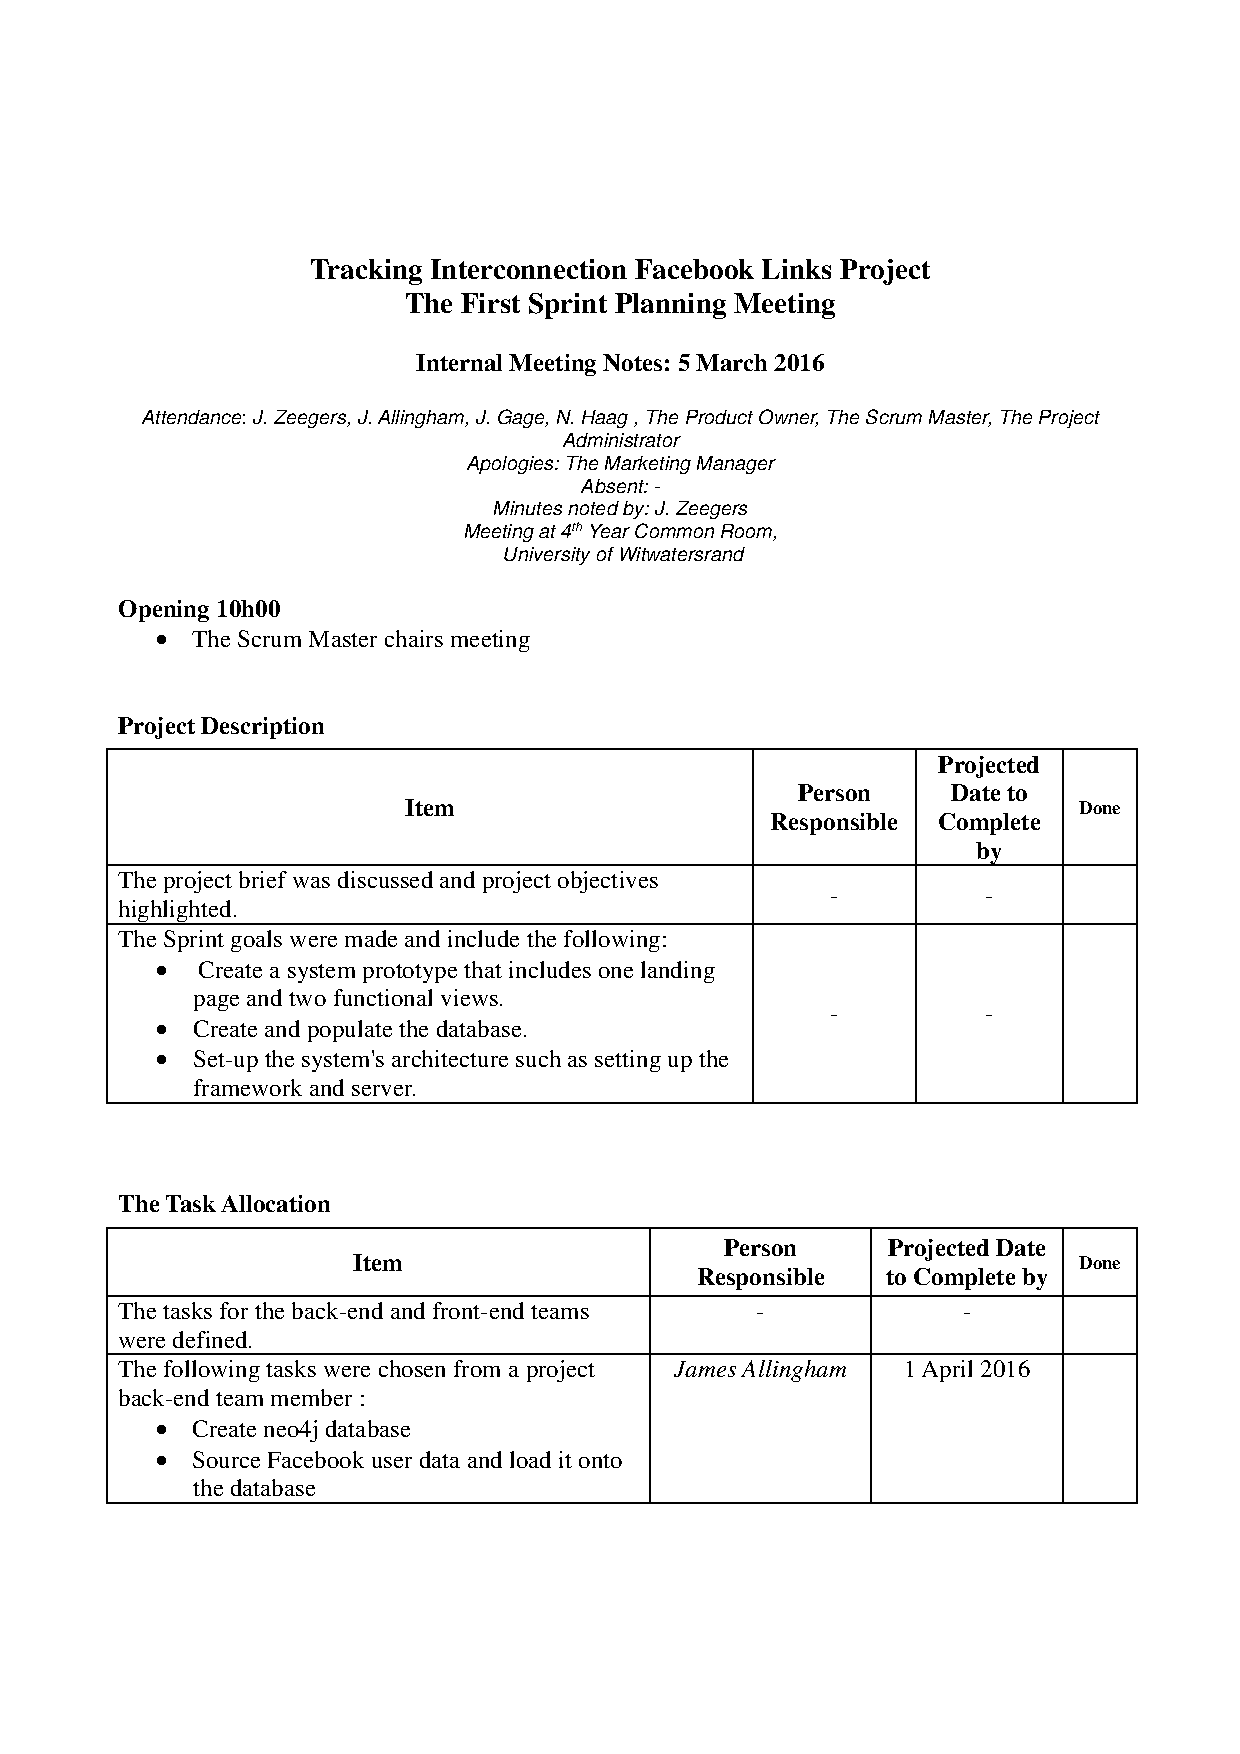
\includepdf[pages=1,pagecommand={\section{The Minutes from the First Sprint Planning Meeting}}, fitpaper=true, scale=0.8]{Minutes.pdf}
	\includepdf[pages=2-,pagecommand={}, fitpaper=true, scale = 0.8]{Minutes.pdf}	

\end{document}